% Biên dịch được với pdfLaTeX (mặc định Overleaf) hoặc XeLaTeX/LuaLaTeX.
% Hình: trên Overleaf đặt trong figures_A (outputs/a7/figures) và figures_B (outputs/b6/figures).
% Logo trường: đặt file logo_uet.png cùng thư mục với file .tex này.
\documentclass[11pt,a4paper]{article}

\usepackage{iftex}
\ifPDFTeX
  \usepackage[utf8]{inputenc}
  \usepackage[T5]{fontenc}
  \usepackage{lmodern}
\else
  \usepackage{fontspec}
\fi
\usepackage{amssymb}
\usepackage{graphicx}
\usepackage{xcolor}
\usepackage[margin=2.2cm]{geometry}
\usepackage{tabularx}
\usepackage{booktabs}
\usepackage{array}
\usepackage{enumitem}
\usepackage{parskip}
\usepackage{float}
\usepackage{tikz}
\usetikzlibrary{shapes.geometric, arrows.meta, positioning, fit, backgrounds, calc}
\usepackage{hyperref}
\hypersetup{unicode=true, colorlinks=true, linkcolor=blue!65!black,
            urlcolor=blue!65!black, citecolor=blue!65!black}

\graphicspath{{figures_A/}{figures_B/}{../outputs/a7/figures/}{../outputs/b6/figures/}}
\renewcommand{\tablename}{Bảng}
\renewcommand{\figurename}{Hình}
\renewcommand{\contentsname}{Mục lục}
\emergencystretch=3em

\definecolor{primaryblue}{RGB}{30, 80, 180}
\definecolor{softblue}{RGB}{236, 243, 255}
\definecolor{softteal}{RGB}{230, 247, 245}
\definecolor{softorange}{RGB}{255, 243, 230}
\definecolor{softgreen}{RGB}{233, 247, 239}
\definecolor{softpurple}{RGB}{244, 236, 255}
\definecolor{darkgray}{RGB}{60, 60, 60}
\tikzset{
  box/.style={rectangle, rounded corners=4pt, draw=primaryblue!80!black, thick, fill=softblue,
              align=center, text width=2.4cm, minimum height=11mm, inner sep=4pt, font=\small},
  boxteal/.style={box, draw=teal!80!black, fill=softteal},
  boxorange/.style={box, draw=orange!80!black, fill=softorange},
  boxpurple/.style={box, draw=purple!80!black, fill=softpurple},
  boxgreen/.style={box, draw=green!60!black, fill=softgreen},
  arr/.style={-{Latex[length=2.4mm, width=1.6mm]}, thick, color=darkgray},
  und/.style={thick, color=darkgray},
  lbl/.style={font=\footnotesize, fill=white, inner sep=1.5pt},
}

\newcommand{\tenhocphan}{Phân tích mạng phương tiện xã hội trong kinh doanh}
\newcommand{\giangvien}{TS. Trần Mai Vũ}
\newcommand{\lophoc}{INT3235E\_1}
\newcommand{\linkgithub}{https://github.com/Sntug/FinalTerm}

\begin{document}

\begin{titlepage}
\centering
{\Large\bfseries TRƯỜNG ĐẠI HỌC CÔNG NGHỆ\par}
{\Large\bfseries ĐẠI HỌC QUỐC GIA HÀ NỘI\par}
\vspace{1.2cm}
\IfFileExists{logo_uet.png}{\includegraphics[height=3.6cm]{logo_uet.png}\par}{}
\vspace{1.5cm}
{\LARGE\bfseries BÁO CÁO BÀI TẬP CUỐI KỲ\par}
\vspace{5mm}
{\large Học phần: \tenhocphan\par}
\vspace{1.5cm}
{\LARGE\bfseries Đề tài 30: Mạng lưới các tác giả và tổ chức nghiên cứu\\[4pt] về Thị giác máy tính (Computer Vision)\par}
\vspace{2cm}
\begin{tabular}{@{}ll@{}}
Giảng viên: & \giangvien\\
Lớp: & \lophoc\\[6pt]
Sinh viên: & Đinh Tiến Hùng -- 23020538\\
 & Nông Sơn Tùng -- 23020571\\[6pt]
Mã nguồn: & \url{\linkgithub}\\
\end{tabular}
\vfill
{\large Hà Nội, tháng 11 năm 2026\par}
\end{titlepage}

\tableofcontents
\newpage


\section{Giới thiệu và phân công}

\subsection{Mục tiêu và phạm vi}
Nhóm xây dựng mạng xã hội học thuật của cộng đồng Thị giác máy tính từ dữ liệu bài báo. Mạng cho biết ai viết chung với ai, họ thuộc tổ chức và quốc gia nào, bài nào trích dẫn bài nào, và mỗi bài nghiên cứu bài toán gì, dùng phương pháp gì, thử nghiệm trên tập dữ liệu nào.

Mẫu gồm 700 bài thuộc hội nghị chính (main conference): 350 bài CVPR 2024 và 350 bài ICCV 2023. Dữ liệu lấy từ CVF Open Access và bổ sung bằng OpenAlex, lưu trong Neo4j và phân tích bằng NetworkX.

\subsection{Đối chiếu yêu cầu đề bài}
\begin{table}[H]
\small\centering
\renewcommand{\arraystretch}{1.2}
\caption{Yêu cầu của đề bài và kết quả đạt được}
\label{tab:yeucau}
\begin{tabularx}{\textwidth}{@{}>{\raggedright\arraybackslash}p{4.2cm} >{\raggedright\arraybackslash}X >{\raggedright\arraybackslash}p{3.6cm}@{}}
\toprule
\textbf{Yêu cầu} & \textbf{Kết quả} & \textbf{Chi tiết}\\
\midrule
Tối thiểu 2000 nút & 4182 nút, 8 loại nút & Bảng~\ref{tab:a6}\\
Tối thiểu 5000 cạnh & 16979 cạnh & Bảng~\ref{tab:a6}\\
Tối thiểu 10 loại quan hệ & 10 loại quan hệ, cạnh nào cũng có nguồn gốc & Bảng~\ref{tab:b1}\\
Dữ liệu bài báo khoa học & CVF Open Access, OpenAlex; arXiv và Crossref để đối chiếu & Mục~\ref{sec:nguon}\\
Lưu trong CSDL đồ thị & Neo4j Community; nạp lại nhiều lần không sinh trùng & Mục~\ref{sec:neo4j}\\
\bottomrule
\end{tabularx}
\end{table}

\subsection{Phân công công việc}

\begin{table}[H]
\small\centering
\renewcommand{\arraystretch}{1.25}
\caption{Phân công công việc trong nhóm}
\label{tab:phancong}
\begin{tabularx}{\textwidth}{@{}>{\raggedright\arraybackslash}p{3.2cm} >{\raggedright\arraybackslash}X >{\raggedright\arraybackslash}X@{}}
\toprule
\textbf{Hạng mục} & \textbf{A: Đinh Tiến Hùng (23020538)} & \textbf{B: Nông Sơn Tùng (23020571)}\\
\midrule
Dữ liệu phụ trách & 350 bài CVPR 2024 & 350 bài ICCV 2023\\
Thu thập & Viết bộ thu thập dùng chung cho CVF và OpenAlex; thu 350 bài CVPR & Dựng repo GitHub và Neo4j; thu 350 bài ICCV\\
Tiền xử lý & Viết bộ làm sạch và ghép định danh tác giả, tổ chức; đối chiếu với arXiv, Crossref & Làm sạch dữ liệu ICCV, rà các trường hợp chưa rõ\\
NLP & Luật trích Task và Dataset & Luật trích Method; chạy cả ba nhóm luật trên 700 bài\\
Graph và CSDL & Bộ kiểm tra dữ liệu trước khi dựng graph & Nạp Neo4j; dựng cạnh đồng tác giả và hợp tác tổ chức\\
Phân tích & Thống kê độ đầy đủ dữ liệu và kết quả Task/Dataset & Phân tích mạng: cộng đồng, PageRank, trích dẫn giữa nhóm, case study, truy vấn Cypher\\
Chất lượng & Kiểm tra tự động, lấy mẫu chấm; chấm nửa mẫu A & Chấm nửa mẫu B, đọc chéo\\
Báo cáo & Phần nguồn dữ liệu, tiền xử lý, NLP & Phần mô hình mạng, Neo4j, kết quả; gộp báo cáo\\
\bottomrule
\end{tabularx}
\end{table}

Cả hai cùng thống nhất lược đồ graph, định dạng dữ liệu trao đổi giữa hai phần, cách đếm nút và cạnh, và rà chéo dữ liệu của nhau trước khi gộp.


\section{Mô hình mạng}\label{sec:mohinh}

\subsection{Nút, cạnh và cách đếm}\label{sec:b2.1}

Graph có 8 loại nút và 10 loại quan hệ, tổng cộng 4182 nút và 16979 cạnh. Tác giả và tổ chức là trọng tâm phân tích; Paper, kỳ hội nghị, Task, Method, Dataset và quốc gia bổ sung bối cảnh. Hình~\ref{fig:schema} là lược đồ, Bảng~\ref{tab:b1} mô tả từng quan hệ.

\begin{figure}[H]
\centering
\resizebox{\textwidth}{!}{%
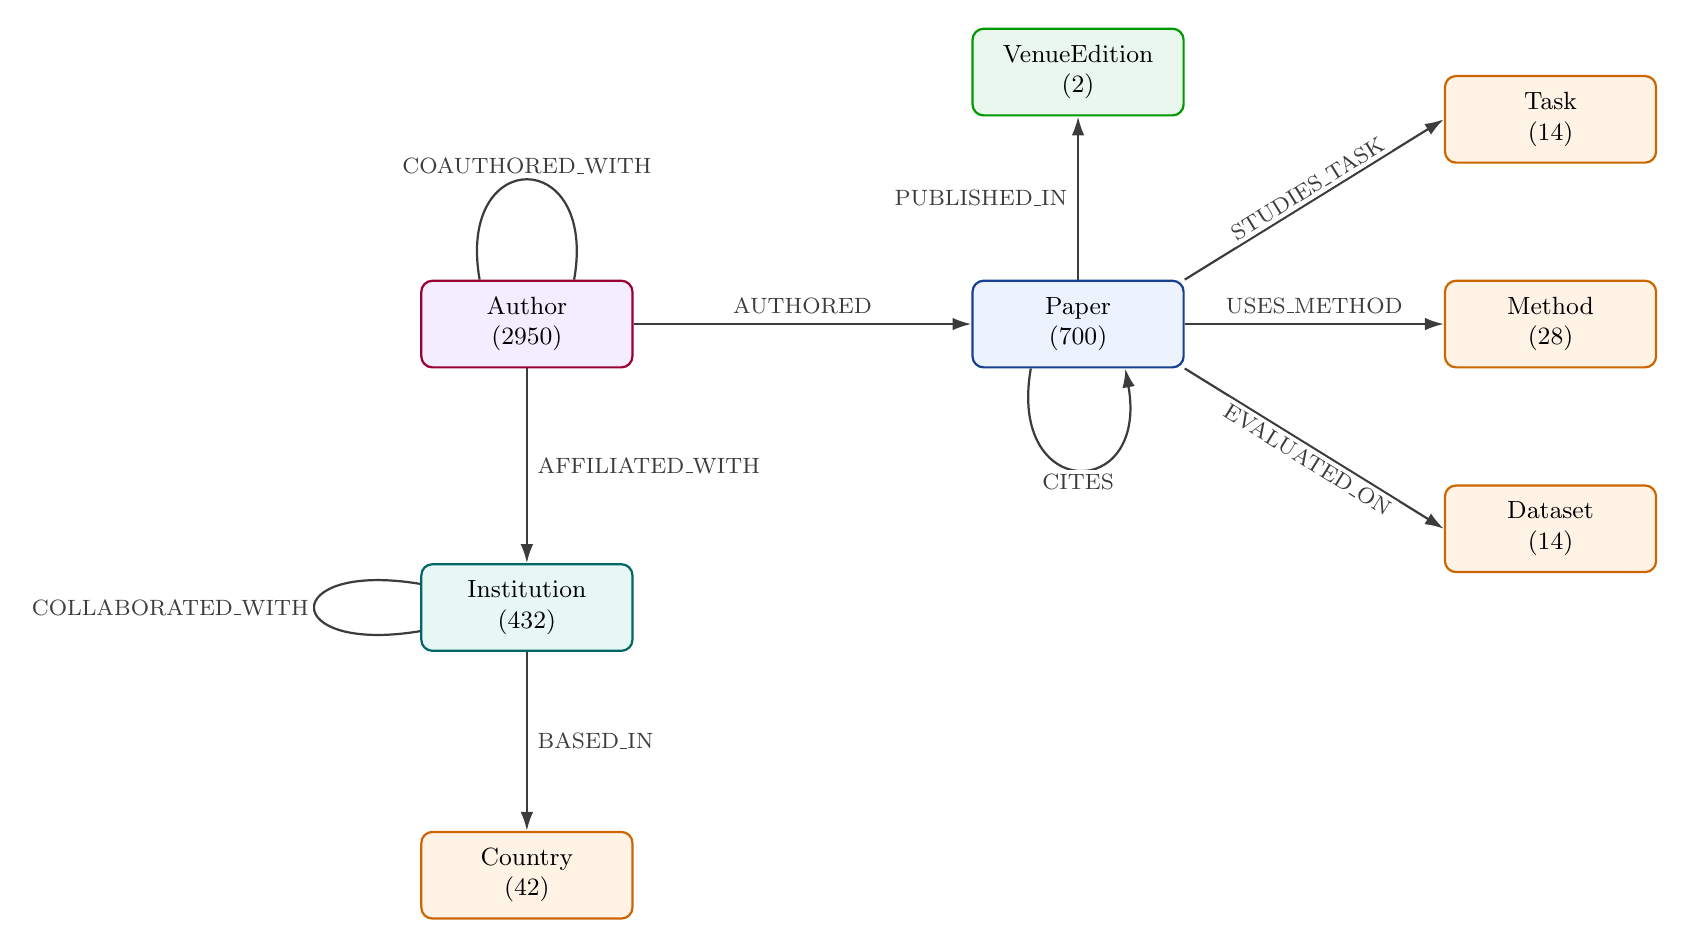
\begin{tikzpicture}
  \node[boxpurple] (author)  at (0,0)    {Author\\(2950)};
  \node[box]       (paper)   at (7,0)    {Paper\\(700)};
  \node[boxgreen]  (venue)   at (7,3.2)  {VenueEdition\\(2)};
  \node[boxteal]   (inst)    at (0,-3.6) {Institution\\(432)};
  \node[boxorange] (country) at (0,-7)   {Country\\(42)};
  \node[boxorange] (task)    at (13,2.6) {Task\\(14)};
  \node[boxorange] (method)  at (13,0)   {Method\\(28)};
  \node[boxorange] (dataset) at (13,-2.6){Dataset\\(14)};

  \draw[arr] (author) -- node[lbl, above=2pt] {AUTHORED} (paper);
  \draw[arr] (author) -- node[lbl, right=2pt] {AFFILIATED\_WITH} (inst);
  \draw[arr] (inst) -- node[lbl, right=2pt] {BASED\_IN} (country);
  \draw[arr] (paper) -- node[lbl, left=2pt] {PUBLISHED\_IN} (venue);
  \draw[arr] (paper.north east) -- node[lbl, above, sloped] {STUDIES\_TASK} (task.west);
  \draw[arr] (paper.east) -- node[lbl, above=2pt] {USES\_METHOD} (method.west);
  \draw[arr] (paper.south east) -- node[lbl, below, sloped] {EVALUATED\_ON} (dataset.west);

  \draw[arr] ([xshift=-6mm]paper.south) .. controls +(-0.3,-1.7) and +(0.3,-1.7) .. node[lbl, below] {CITES} ([xshift=6mm]paper.south);
  \draw[und] ([xshift=-6mm]author.north) .. controls +(-0.3,1.7) and +(0.3,1.7) .. node[lbl, above] {COAUTHORED\_WITH} ([xshift=6mm]author.north);
  \draw[und] ([yshift=3mm]inst.west) .. controls +(-1.8,0.3) and +(-1.8,-0.3) .. node[lbl, left] {COLLABORATED\_WITH} ([yshift=-3mm]inst.west);
\end{tikzpicture}}
\caption{Lược đồ graph: 8 loại nút (số nút trong ngoặc) và 10 loại quan hệ. Mũi tên là quan hệ có hướng; đường không mũi tên là quan hệ vô hướng.}
\label{fig:schema}
\end{figure}

\begin{table}[H]
\footnotesize\centering
\renewcommand{\arraystretch}{1.2}
\caption{Mười loại quan hệ trong graph}
\label{tab:b1}
\begin{tabularx}{\textwidth}{@{}l >{\raggedright\arraybackslash}p{3.2cm} l r >{\raggedright\arraybackslash}X@{}}
\toprule
\textbf{Quan hệ} & \textbf{Hướng} & \textbf{Cách tạo} & \textbf{Số cạnh} & \textbf{Ý nghĩa}\\
\midrule
AUTHORED & Author $\to$ Paper & dữ liệu nguồn & 3282 & tác giả đứng tên trên bài\\
AFFILIATED\_\allowbreak WITH & Author $\to$ Institution & dữ liệu nguồn & 3237 & tổ chức tác giả ghi trên bài\\
PUBLISHED\_\allowbreak IN & Paper $\to$ VenueEdition & dữ liệu nguồn & 700 & bài thuộc kỳ hội nghị nào\\
CITES & Paper $\to$ Paper & dữ liệu nguồn & 97 & bài này trích dẫn bài kia (cả hai trong mẫu)\\
BASED\_\allowbreak IN & Institution $\to$ Country & dữ liệu nguồn & 432 & tổ chức đặt ở nước nào\\
COAUTHORED\_\allowbreak WITH & Author $\leftrightarrow$ Author & suy ra & 7771 & hai người cùng đứng tên; trọng số là số bài chung\\
COLLABORATED\_\allowbreak WITH & Institution $\leftrightarrow$ Institution & suy ra & 1140 & hai tổ chức có tác giả viết chung; trọng số là số bài chung\\
STUDIES\_\allowbreak TASK & Paper $\to$ Task & NLP & 97 & bài nghiên cứu bài toán nào\\
EVALUATED\_\allowbreak ON & Paper $\to$ Dataset & NLP & 28 & bài thử nghiệm trên tập dữ liệu nào\\
USES\_\allowbreak METHOD & Paper $\to$ Method & NLP & 195 & bài dùng phương pháp nào\\
\bottomrule
\end{tabularx}
\end{table}

{\footnotesize ``Dữ liệu nguồn'': lấy trực tiếp từ CVF/OpenAlex. ``Suy ra'': tính từ các quan hệ AUTHORED và AFFILIATED\_WITH. ``NLP'': trích từ tiêu đề và abstract (Mục~\ref{sec:nlp}). Cạnh nào cũng lưu kèm bài và nguồn làm căn cứ.\par}

Một số quy ước khi đếm:
\begin{itemize}[leftmargin=1.4em]
  \item Mỗi cặp tác giả (hoặc cặp tổ chức) chỉ có một cạnh, không có cạnh tự nối. Trọng số là số bài khác nhau mà cặp đó cùng xuất hiện. Trong 7771 cạnh đồng tác giả, 7681 cạnh có trọng số 1, 85 cạnh trọng số 2, 4 cạnh trọng số 3 và 1 cạnh trọng số 4.
  \item Một tác giả ghi hai tổ chức không tạo cạnh hợp tác giữa hai tổ chức đó; cần hai tác giả khác nhau. Cạnh hợp tác tổ chức chỉ phản ánh việc viết chung bài, không khẳng định có thỏa thuận hợp tác chính thức.
  \item Graph chỉ chứa 700 bài của mẫu. Bài được trích dẫn mà nằm ngoài mẫu không được thêm thành nút, nên CITES chỉ nối các bài trong mẫu với nhau.
  \item Mỗi nút có ID riêng kèm tiền tố theo loại, ví dụ \texttt{author:openalex:\ldots}, \texttt{country:CN}, \texttt{task:object-detection}. Tên hiển thị không dùng làm khóa. Country là nước của \emph{tổ chức} tác giả ghi trên bài, không phải quốc tịch tác giả.
\end{itemize}


\section{Nguồn dữ liệu và công nghệ}

\subsection{Nguồn dữ liệu}\label{sec:nguon}

700 bài là mẫu nhóm tự chọn, không phải toàn bộ bài của hai hội nghị và không đại diện cho cả ngành.

\begin{table}[H]
\small\centering
\renewcommand{\arraystretch}{1.25}
\caption{Các nguồn dữ liệu và vai trò}
\label{tab:nguon}
\begin{tabularx}{\textwidth}{@{}>{\raggedright\arraybackslash}p{3.2cm} >{\raggedright\arraybackslash}X@{}}
\toprule
\textbf{Nguồn} & \textbf{Dùng để lấy}\\
\midrule
\href{https://openaccess.thecvf.com/}{CVF Open Access} & Danh sách bài hội nghị chính của \href{https://openaccess.thecvf.com/CVPR2024}{CVPR 2024} và \href{https://openaccess.thecvf.com/ICCV2023}{ICCV 2023} (bỏ bài workshop); tiêu đề, danh sách tác giả theo thứ tự, abstract, đường dẫn bài.\\
\href{https://help.openalex.org/data/works/}{OpenAlex} & DOI, ID tác giả, tổ chức tác giả ghi trên từng bài, quốc gia của tổ chức, danh sách tài liệu tham khảo. Tổ chức lấy theo \href{https://help.openalex.org/data/authorships/}{từng lần đứng tên trên bài}, không lấy nơi làm việc hiện tại.\\
\href{https://info.arxiv.org/help/versions.html}{arXiv}, \href{https://www.crossref.org/documentation/retrieve-metadata/rest-api/}{Crossref} & Chỉ dùng để đối chiếu một số bài (bản preprint, DOI); không thêm bài mới.\\
\bottomrule
\end{tabularx}
\end{table}

Một bài được nhận vào mẫu khi xác minh được tiêu đề, danh sách tác giả, đúng kỳ hội nghị và đường dẫn. Thiếu DOI, abstract hay tổ chức không làm bài bị loại. Mọi phản hồi từ CVF và OpenAlex được lưu lại, nên toàn bộ quy trình chạy lại được mà không cần mạng.

\begin{table}[H]
\small\centering
\renewcommand{\arraystretch}{1.2}
\caption{Quy mô dữ liệu sau tiền xử lý theo hội nghị}
\label{tab:a1}
\begin{tabularx}{\textwidth}{@{}>{\raggedright\arraybackslash}X l l@{}}
\toprule
\textbf{Chỉ tiêu} & \textbf{CVPR 2024 (A)} & \textbf{ICCV 2023 (B)}\\
\midrule
Bài báo & 350 & 350\\
Tác giả có ID & 1550 & 1546\\
Tổ chức có ID & 294 & 300\\
Lượt đứng tên (một tác giả trên một bài) & 1968 & 1853\\
Cặp (lượt đứng tên, tổ chức) & 2109 & 2275\\
\bottomrule
\end{tabularx}
\end{table}

\subsection{Công nghệ sử dụng}\label{sec:stack}
\begin{table}[H]
\small\centering
\renewcommand{\arraystretch}{1.25}
\caption{Công nghệ sử dụng theo từng khâu}
\label{tab:stack}
\begin{tabularx}{\textwidth}{@{}>{\raggedright\arraybackslash}p{2.8cm} >{\raggedright\arraybackslash}p{4.4cm} >{\raggedright\arraybackslash}X@{}}
\toprule
\textbf{Khâu} & \textbf{Công nghệ} & \textbf{Vai trò}\\
\midrule
Thu thập & Python 3.12 (thư viện chuẩn) & Đọc trang CVF và API OpenAlex; tự thử lại khi lỗi mạng; lưu bản gốc để chạy lại offline.\\
Làm sạch & Python 3.12, CSV/JSONL & Chuẩn hóa văn bản, ghép bài và tác giả giữa các nguồn, ghi lại mọi quyết định ghép.\\
NLP & spaCy 3.8 & Tách câu, so khớp từ điển và luật ngữ cảnh. Không dùng mô hình học máy nên mỗi cạnh đều chỉ ra được câu gốc và luật đã dùng.\\
Lưu trữ graph & Neo4j Community, Cypher & Lưu nút, cạnh và thuộc tính; truy vấn minh họa.\\
Phân tích mạng & NetworkX 3.4, NumPy, SciPy & Degree, thành phần liên thông, hệ số phân cụm, Louvain, PageRank.\\
Trực quan hóa & Matplotlib & Vẽ các hình trong báo cáo.\\
Kiểm thử & \texttt{unittest} & Kiểm tra chất lượng dữ liệu, việc nạp và phân tích.\\
Quản lý mã nguồn & Git, GitHub & Một repo chung, mỗi công việc một nhánh và pull request.\\
\bottomrule
\end{tabularx}
\end{table}

Nhóm chọn Neo4j vì dữ liệu vốn là đồ thị có nhãn và thuộc tính, Cypher viết truy vấn đường đi (tác giả, bài, tổ chức, quốc gia) ngắn gọn, và có thể đọc dữ liệu sang Python để chạy thuật toán bằng NetworkX. Bản Neo4j Community không có sẵn thư viện thuật toán đồ thị, nên phần tính toán chạy bằng NetworkX.

\subsection{Lưu trữ trên Neo4j}\label{sec:neo4j}

Dữ liệu graph được xuất ra file CSV rồi nạp vào Neo4j theo các bước sau:
\begin{enumerate}[leftmargin=1.6em]
  \item Kiểm tra file đầu vào: đủ file, đúng phiên bản, chỉ chứa các loại nút và quan hệ đã thống nhất.
  \item Xóa dữ liệu cũ của dự án và ghi dữ liệu mới. Việc xóa và ghi nằm trong cùng một lần ghi (giao dịch): hoặc thành công toàn bộ, hoặc không thay đổi gì.
  \item Trước khi xác nhận, đếm lại số nút và cạnh trong Neo4j và so với file. Nếu lệch, toàn bộ lần ghi bị hủy, cơ sở dữ liệu giữ nguyên như trước.
\end{enumerate}

Nhờ vậy nạp lại nhiều lần không sinh nút hay cạnh trùng. Mỗi loại nút có ràng buộc ID duy nhất. Hiện Neo4j chứa đúng 4182 nút và 16979 cạnh, khớp với file. Bước phân tích đọc dữ liệu từ Neo4j và tự kiểm tra lại điều này trước khi tính, nên mọi số liệu trong báo cáo ứng với cùng một phiên bản dữ liệu.


\section{Tiền xử lý dữ liệu}

\subsection{Thu thập và làm sạch}\label{sec:tienxuly}

\textbf{Thu thập.} Từ danh sách bài hội nghị chính trên CVF, mỗi kỳ chọn 350 bài theo một thứ tự cố định để lần sau chạy lại vẫn ra đúng các bài đó. Bài không được chọn theo số trích dẫn. Với mỗi bài, bộ thu thập đọc trang chi tiết trên CVF rồi tra thêm trên OpenAlex.

\textbf{Làm sạch.} Bảng~\ref{tab:lamsach} tóm tắt cách xử lý từng loại thực thể. Nguyên tắc chung: chỉ ghép hai bản ghi khi có căn cứ rõ ràng, trường hợp chưa chắc chắn thì giữ riêng và đưa vào danh sách cần xem lại.

\begin{table}[H]
\small\centering
\renewcommand{\arraystretch}{1.25}
\caption{Cách làm sạch và ghép dữ liệu}
\label{tab:lamsach}
\begin{tabularx}{\textwidth}{@{}>{\raggedright\arraybackslash}p{2.4cm} >{\raggedright\arraybackslash}X@{}}
\toprule
\textbf{Đối tượng} & \textbf{Cách xử lý}\\
\midrule
Văn bản & Chuẩn hóa mã Unicode, ký tự HTML và khoảng trắng; giữ nguyên dấu và thứ tự tác giả.\\
Bài báo & ID lấy theo đường dẫn CVF. Hai bản ghi chỉ được coi là một bài khi trùng DOI hoặc ID; tiêu đề gần giống chỉ được đánh dấu để xem lại. Nếu có cả bản hội nghị và bản preprint, giữ bản hội nghị.\\
Tác giả & Nhận diện bằng ID OpenAlex (hoặc ORCID hợp lệ). Không gộp hai người chỉ vì trùng tên. Tác giả không có ID vẫn được ghi trong danh sách tác giả của bài, nhưng không trở thành nút và không bị đoán danh tính.\\
Tổ chức & Nhận diện bằng ID OpenAlex hoặc ROR. Lấy theo tổ chức ghi trên chính bài. Không gộp tổ chức mẹ và tổ chức con chỉ vì tên giống nhau.\\
Lịch sử ghép & Mỗi lần ghép hoặc liên kết đều ghi lại lý do, nguồn và dữ liệu trước/sau, để kiểm tra lại được.\\
\bottomrule
\end{tabularx}
\end{table}

Không có bài nào bị trùng hay xung đột ID ở cả hai hội nghị. Sau khi gộp hai phần, graph có 700 bài, 2950 tác giả, 432 tổ chức và 3821 lượt đứng tên. 146 tác giả và 162 tổ chức xuất hiện ở cả hai hội nghị.

\subsection{Trích xuất Task, Method, Dataset bằng NLP}\label{sec:nlp}

Mục tiêu là đọc tiêu đề và abstract của mỗi bài rồi trả lời ba câu hỏi: bài giải bài toán gì (Task), dùng phương pháp gì (Method), thử nghiệm trên tập dữ liệu nào (Dataset). Nhóm không đọc toàn văn PDF. Cách làm gồm hai bước:

\begin{enumerate}[leftmargin=1.6em]
  \item \textbf{Tìm thuật ngữ.} Dùng từ điển gồm 15 Task, 30 Method và 30 Dataset, mỗi mục có các cách viết khác nhau (ví dụ ``ViT'' và ``Vision Transformer''). spaCy tách abstract thành câu và tìm các thuật ngữ này.
  \item \textbf{Xét ngữ cảnh câu.} Chỉ thấy tên thuật ngữ là chưa đủ. Câu chứa thuật ngữ phải khớp một luật ``nhận'' và không dính luật ``loại'' trong Bảng~\ref{tab:luat}.
\end{enumerate}


\begin{table}[H]
\small\centering
\renewcommand{\arraystretch}{1.25}
\caption{Luật nhận và luật loại khi trích quan hệ}
\label{tab:luat}
\begin{tabularx}{\textwidth}{@{}>{\raggedright\arraybackslash}p{3.4cm} @{\hspace{0.4cm}} >{\raggedright\arraybackslash}X@{}}
\toprule
\textbf{Quan hệ} & \textbf{Nhận khi}\\
\midrule
STUDIES\_TASK & Tên bài toán có trong tiêu đề, hoặc abstract có câu dạng ``we / this paper + giải quyết + bài toán'' (ví dụ ``we address \ldots{} object detection'').\\
EVALUATED\_ON & Câu nói về thí nghiệm hoặc kết quả trên tập dữ liệu, ví dụ ``experiments on nuScenes show \ldots''. Chỉ nhắc tên tập dữ liệu thì không tính.\\
USES\_METHOD & Tên phương pháp có trong tiêu đề; hoặc đứng gần động từ ``use / adopt / build \ldots''; hoặc ở dạng ``\ldots-based'' trong câu có ``we / our''.\\
\midrule
\textbf{Loại khi} & Câu phủ định; câu nói về tương lai hoặc giả định; câu nói về công trình trước hoặc phương pháp so sánh; với Dataset, câu nói về huấn luyện hoặc tiền huấn luyện thay vì đánh giá.\\
\bottomrule
\end{tabularx}
\end{table}


Mỗi cạnh lưu kèm câu gốc, vị trí câu trong văn bản và mã luật đã dùng, nên ai cũng có thể mở bài ra kiểm tra lại. Một bài chỉ có một cạnh tới mỗi Task/Method/Dataset, dù nhiều câu cùng nhắc tới. Bảng~\ref{tab:a3} là bốn ví dụ thật.

\begin{table}[H]
\small\centering
\renewcommand{\arraystretch}{1.2}
\caption{Ví dụ thật từ các bài CVPR 2024}
\label{tab:a3}
\begin{tabularx}{\textwidth}{@{}l >{\raggedright\arraybackslash}p{2.6cm} >{\raggedright\arraybackslash}X >{\raggedright\arraybackslash}p{3.6cm}@{}}
\toprule
\textbf{\#} & \textbf{Thuật ngữ} & \textbf{Câu gốc} & \textbf{Kết quả}\\
\midrule
1 & \href{https://openaccess.thecvf.com/content/CVPR2024/html/Li_UniMODE_Unified_Monocular_3D_Object_Detection_CVPR_2024_paper.html}{Object Detection} & UniMODE: Unified Monocular 3D Object Detection (tiêu đề) & Nhận STUDIES\_TASK: thuật ngữ nằm trong tiêu đề\\
2 & \href{https://openaccess.thecvf.com/content/CVPR2024/html/Wei_Editable_Scene_Simulation_for_Autonomous_Driving_via_Collaborative_LLM-Agents_CVPR_2024_paper.html}{Waymo Open Dataset} & Our experiments on Waymo Open Dataset demonstrate that ChatSim can handle complex language commands \ldots{} & Nhận EVALUATED\_ON: câu nói về thí nghiệm\\
3 & \href{https://openaccess.thecvf.com/content/CVPR2024/html/Jain_Towards_Understanding_and_Improving_Adversarial_Robustness_of_Vision_Transformers_CVPR_2024_paper.html}{CIFAR-10} & On incorporating AAS-AT with existing methods we outperform them on VITs over 1.3-3.5\% on CIFAR10. & Loại: có chữ ``existing methods'' (công trình trước)\\
4 & \href{https://openaccess.thecvf.com/content/CVPR2024/html/Yu_Rethinking_the_Evaluation_Protocol_of_Domain_Generalization_CVPR_2024_paper.html}{ImageNet} & \ldots{} supervised pretraining on ImageNet and oracle model selection. \ldots{} & Loại: ImageNet dùng để tiền huấn luyện, không phải đánh giá\\
\bottomrule
\end{tabularx}
\end{table}

Ví dụ 3 cho thấy luật khá thận trọng: câu thật ra có báo kết quả của bài trên CIFAR-10, nhưng vì có cụm ``existing methods'' nên bị loại. Nhóm chấp nhận bỏ sót để đổi lấy độ chính xác cao. Vì vậy, bài không có cạnh Task/Method/Dataset chưa chắc là không liên quan; nó chỉ chưa đủ căn cứ theo luật.

\subsection{Độ đầy đủ của dữ liệu và kết quả NLP}\label{sec:coverage}

\begin{table}[H]
\small\centering
\renewcommand{\arraystretch}{1.2}
\caption{Tỷ lệ thiếu dữ liệu theo trường}
\label{tab:a4}
\begin{tabularx}{\textwidth}{@{}>{\raggedright\arraybackslash}X l l@{}}
\toprule
\textbf{Trường thiếu (trên tổng)} & \textbf{CVPR 2024 (A)} & \textbf{ICCV 2023 (B)}\\
\midrule
Thiếu DOI (trên số bài) & 22/350 (6,29\%) & 0/350 (0,00\%)\\
Thiếu abstract (trên số bài) & 0/350 (0,00\%) & 0/350 (0,00\%)\\
Thiếu ID OpenAlex (trên số bài) & 22/350 (6,29\%) & 0/350 (0,00\%)\\
Thiếu liên kết arXiv (trên số bài) & 140/350 (40,00\%) & 131/350 (37,43\%)\\
Thiếu ID tác giả (trên lượt đứng tên) & 340/1968 (17,28\%) & 199/1853 (10,74\%)\\
Chưa xác định được tổ chức (trên lượt đứng tên) & 466/1968 (23,68\%) & 295/1853 (15,92\%)\\
\bottomrule
\end{tabularx}
\end{table}

\begin{figure}[H]
\centering
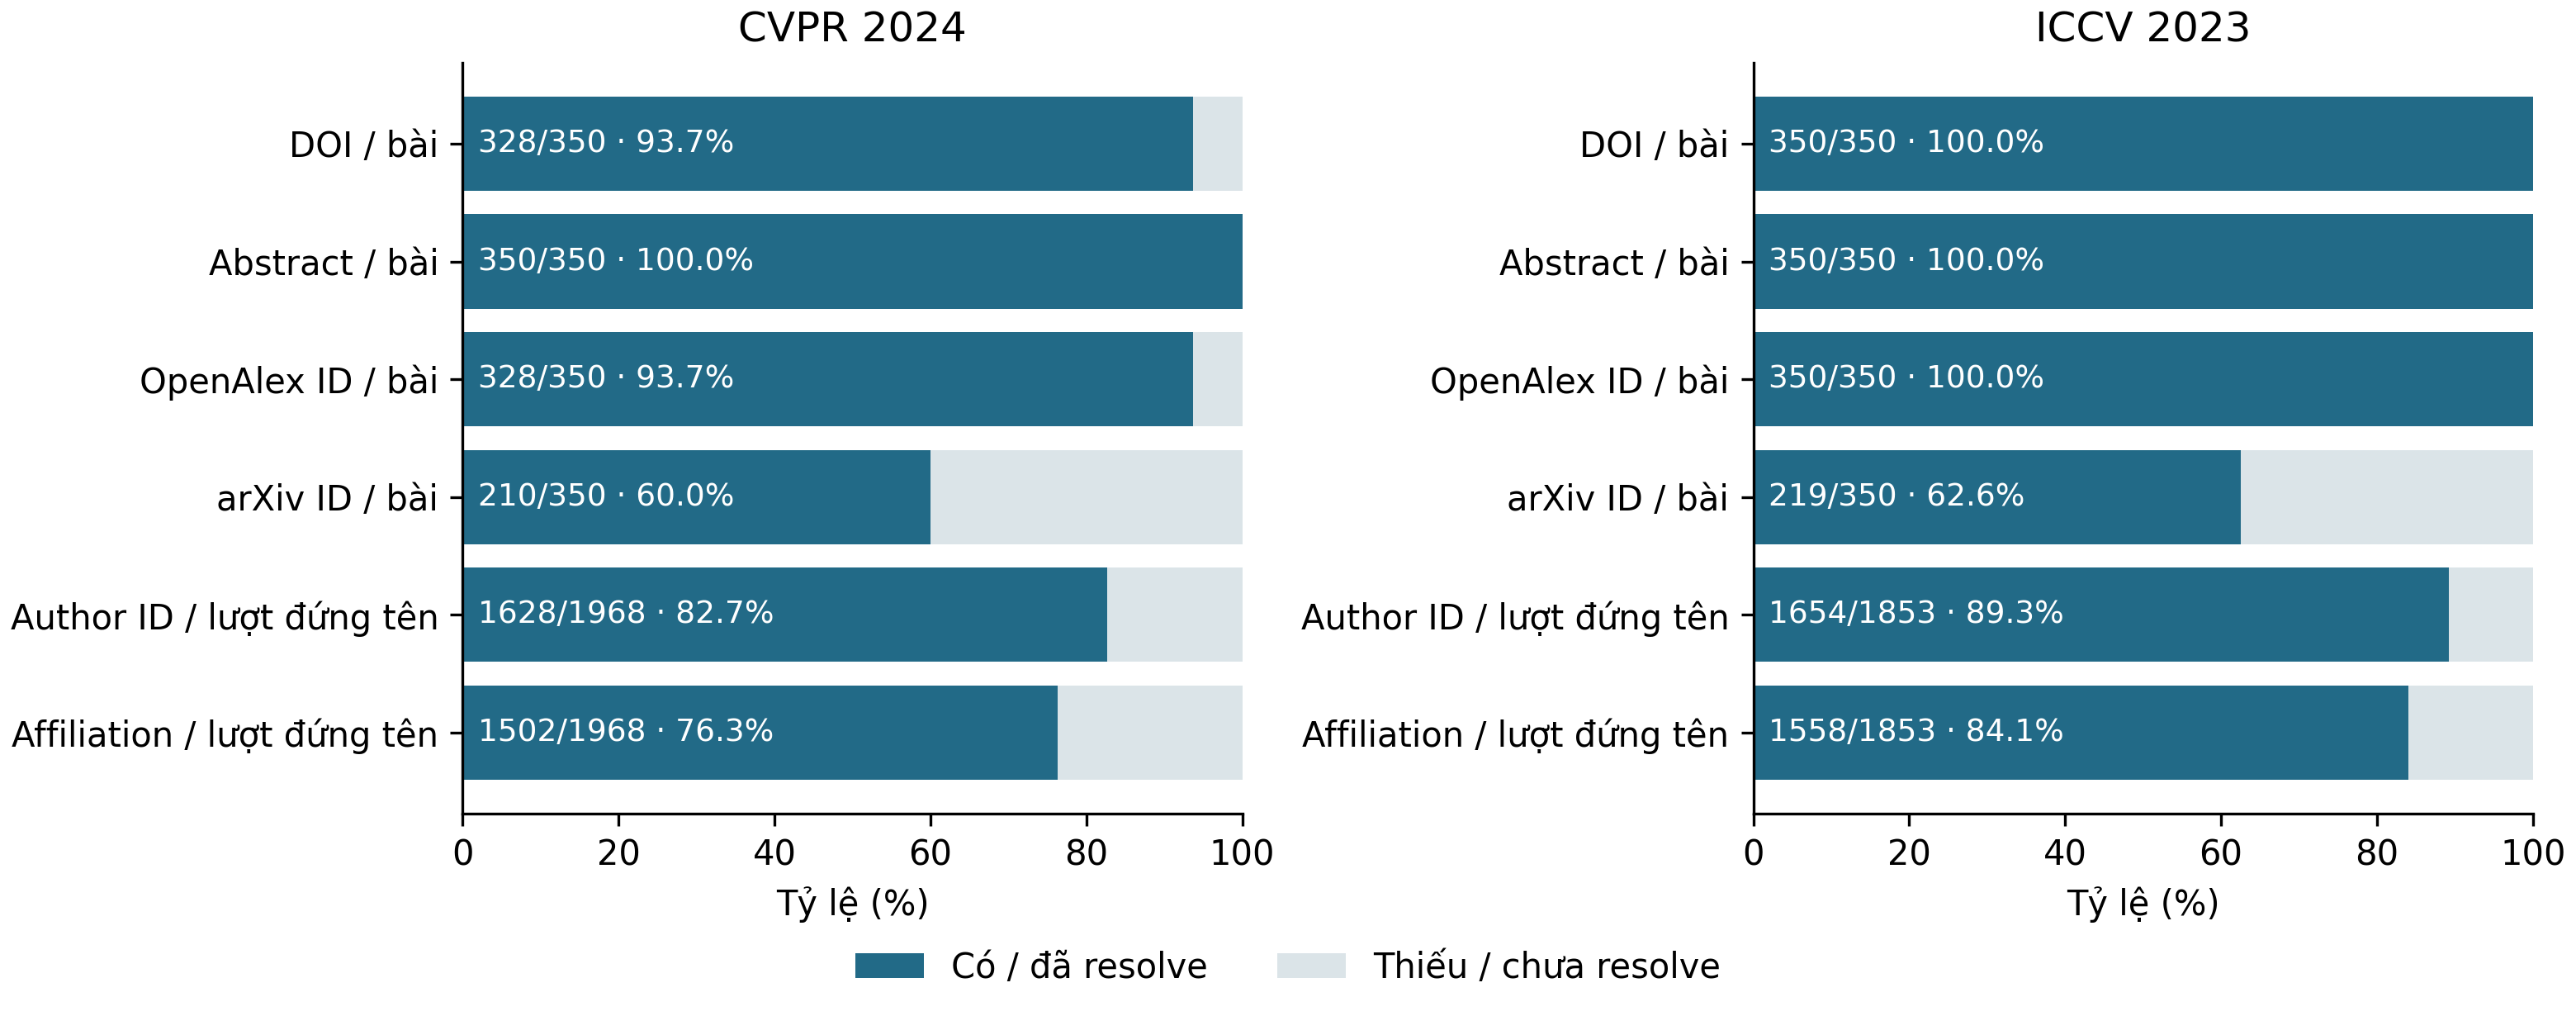
\includegraphics[width=0.92\textwidth]{metadata_coverage.png}
\caption{Độ đầy đủ của dữ liệu theo hội nghị}
\label{fig:a1}
\end{figure}

Bài nào cũng có tiêu đề và abstract, thuận lợi cho NLP. Phần thiếu nhiều nhất là ID tác giả và tổ chức, nhất là ở CVPR. Tác giả thiếu ID không vào được graph, nên mạng hợp tác sẽ nghiêng về những tác giả và tổ chức mà OpenAlex nhận diện tốt. Chênh lệch giữa hai hội nghị ở đây chỉ nói về dữ liệu nguồn, không nói gì về chất lượng bài.

\begin{table}[H]
\small\centering
\renewcommand{\arraystretch}{1.2}
\caption{Kết quả trích Task và Dataset theo hội nghị}
\label{tab:a5}
\begin{tabularx}{\textwidth}{@{}l >{\raggedright\arraybackslash}X >{\raggedright\arraybackslash}X >{\raggedright\arraybackslash}X@{}}
\toprule
\textbf{Quan hệ} & \textbf{CVPR 2024 (A)} & \textbf{ICCV 2023 (B)} & \textbf{Gộp trong graph}\\
\midrule
STUDIES\_TASK & 31 cạnh; 10 Task; 31 bài & 66 cạnh; 13 Task; 64 bài & 97 cạnh; 14 Task\\
EVALUATED\_ON & 9 cạnh; 7 Dataset; 8 bài & 19 cạnh; 9 Dataset; 13 bài & 28 cạnh; 14 Dataset\\
\bottomrule
\end{tabularx}
\end{table}

\begin{figure}[H]
\centering
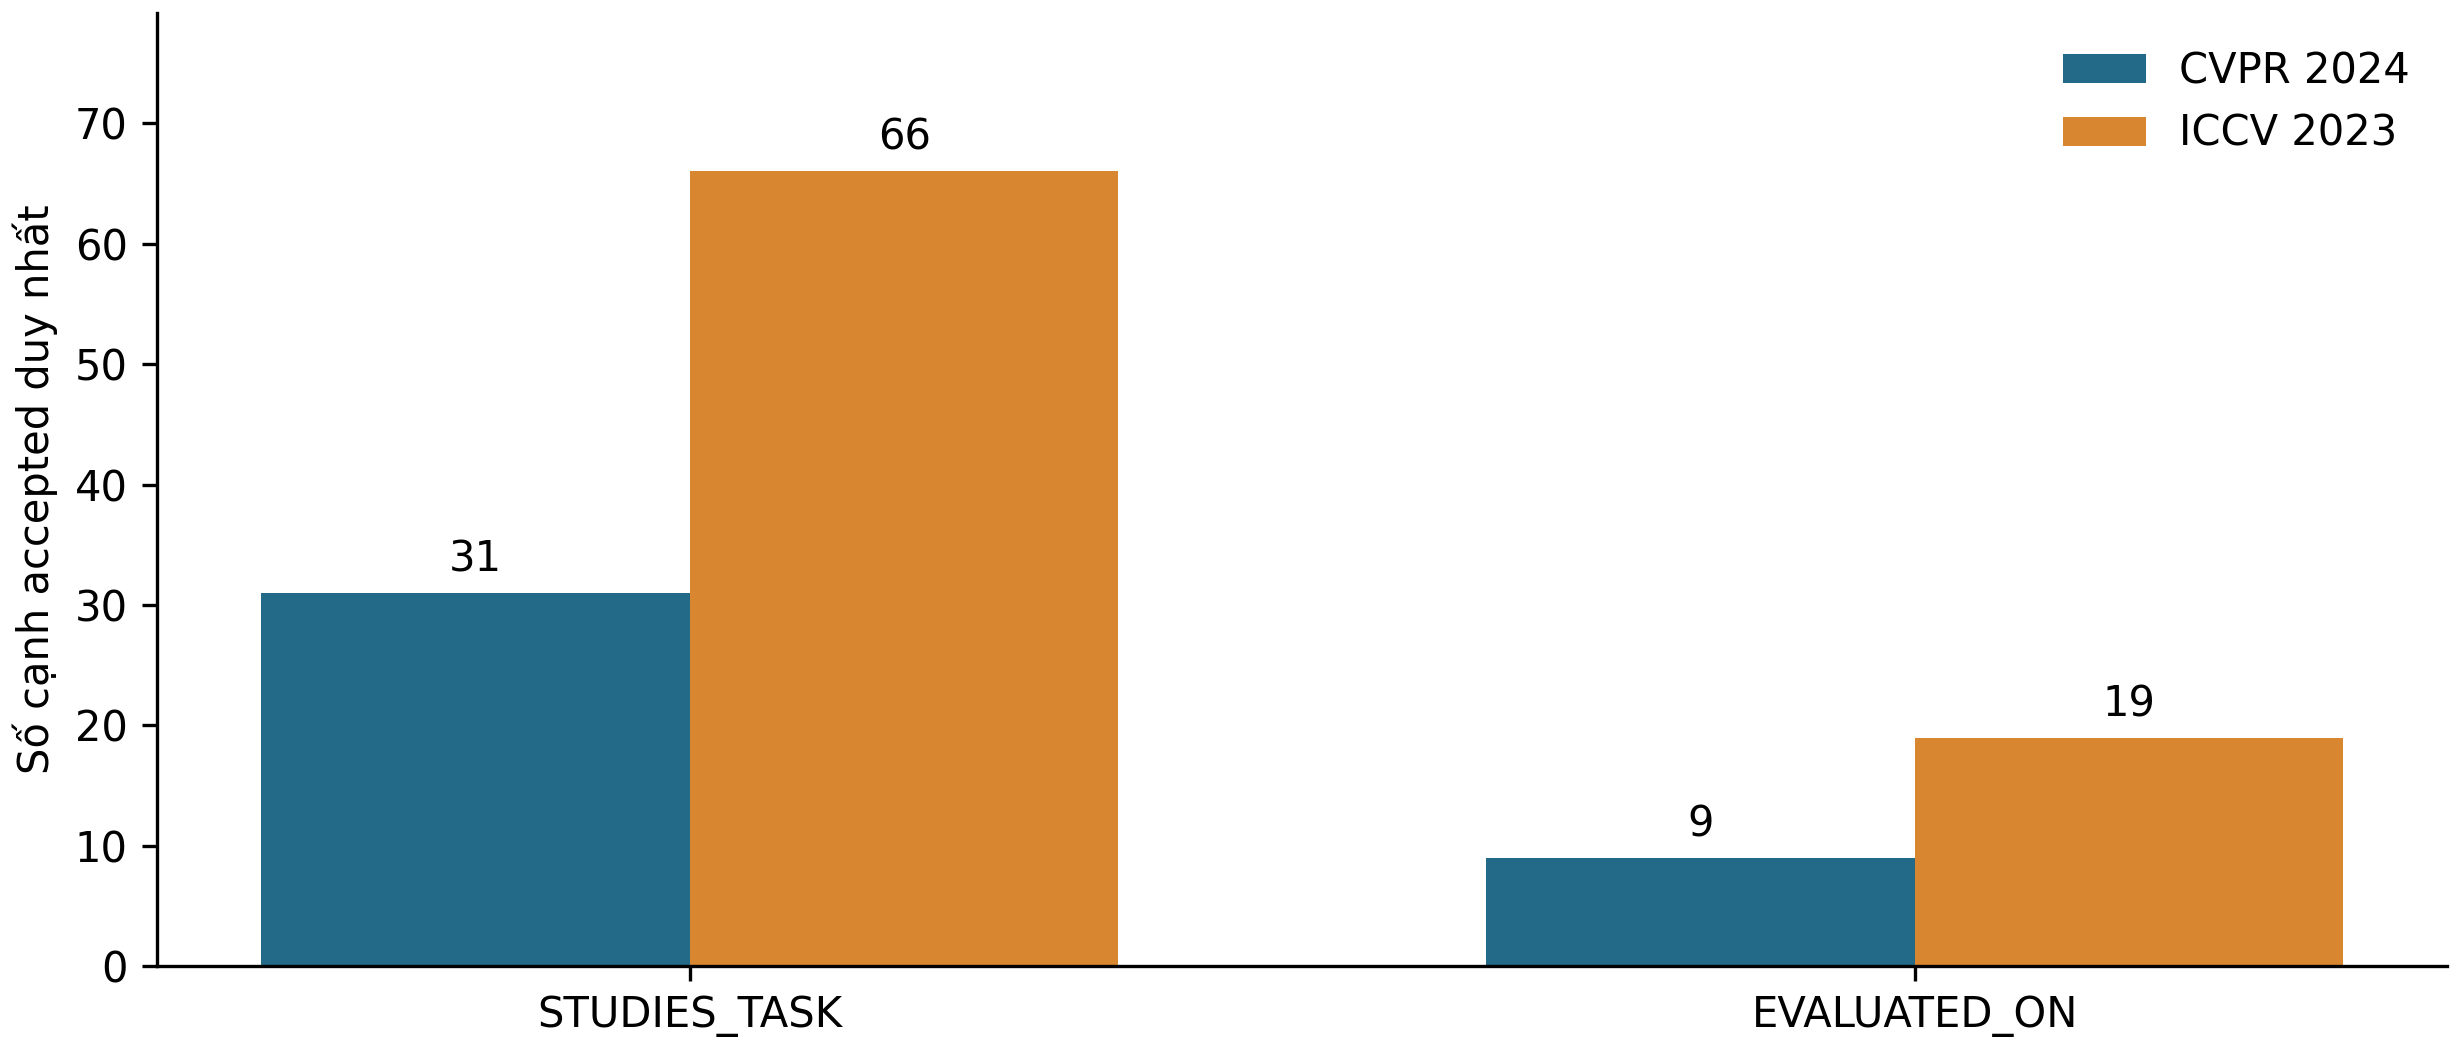
\includegraphics[width=0.92\textwidth]{nlp_relations.png}
\caption{Số cạnh NLP theo hội nghị}
\label{fig:a2}
\end{figure}

USES\_METHOD có 195 cạnh trên 178 bài. Số cạnh nhỏ so với 700 bài vì từ điển có giới hạn và luật thận trọng, nên không dùng để so sánh mức độ phổ biến thật của bài toán giữa hai hội nghị.


\section{Kết quả phân tích mạng}

\subsection{Quy mô graph}\label{sec:quymo}

\begin{table}[H]
\small\centering
\renewcommand{\arraystretch}{1.2}
\caption{Số nút và số cạnh theo loại}
\label{tab:a6}
\begin{tabularx}{\textwidth}{@{}l l >{\raggedright\arraybackslash}X l@{}}
\toprule
\textbf{Loại nút} & \textbf{Số nút} & \textbf{Quan hệ} & \textbf{Số cạnh}\\
\midrule
Author & 2950 & AFFILIATED\_\allowbreak WITH & 3237\\
Country & 42 & AUTHORED & 3282\\
Dataset & 14 & BASED\_\allowbreak IN & 432\\
Institution & 432 & CITES & 97\\
Method & 28 & COAUTHORED\_\allowbreak WITH & 7771\\
Paper & 700 & COLLABORATED\_\allowbreak WITH & 1140\\
Task & 14 & EVALUATED\_\allowbreak ON & 28\\
VenueEdition & 2 & PUBLISHED\_\allowbreak IN & 700\\
 &  & STUDIES\_\allowbreak TASK & 97\\
 &  & USES\_\allowbreak METHOD & 195\\
\midrule
\textbf{Tổng} & \textbf{4182} & & \textbf{16979}\\
\bottomrule
\end{tabularx}
\end{table}

Các chỉ số dưới đây được tính bằng NetworkX trên dữ liệu đọc từ Neo4j. Mạng đồng tác giả và hợp tác tổ chức là đồ thị vô hướng có trọng số; mạng trích dẫn là đồ thị có hướng giữa các bài. Phân cộng đồng dùng thuật toán Louvain (seed 42) trên thành phần liên thông lớn nhất; PageRank dùng hệ số 0,85.

\subsection{Mạng đồng tác giả}\label{sec:b5.2}

\begin{table}[H]
\small\centering
\renewcommand{\arraystretch}{1.2}
\caption{Chỉ số mạng đồng tác giả}
\label{tab:b2}
\begin{tabularx}{\textwidth}{@{}>{\raggedright\arraybackslash}X >{\raggedright\arraybackslash}X@{}}
\toprule
\textbf{Chỉ số} & \textbf{Giá trị}\\
\midrule
Số tác giả / số cặp đồng tác giả & 2950 / 7771\\
Mật độ & 0,0018\\
Degree: trung bình / trung vị / p90 / lớn nhất & 5,27 / 5 / 9 / 41\\
Strength (có tính trọng số): trung bình / lớn nhất & 5,33 / 45\\
Tác giả không nối với ai & 4\\
Số thành phần liên thông (có hơn 1 tác giả) & 416 (412)\\
Thành phần lớn nhất & 502 tác giả (17,0\%), 1936 cạnh\\
Hệ số phân cụm trung bình (toàn mạng / thành phần lớn nhất) & 0,921 / 0,908\\
Louvain trên thành phần lớn nhất & 19 cộng đồng, modularity 0,867\\
\bottomrule
\end{tabularx}
\end{table}

\begin{figure}[H]
\centering
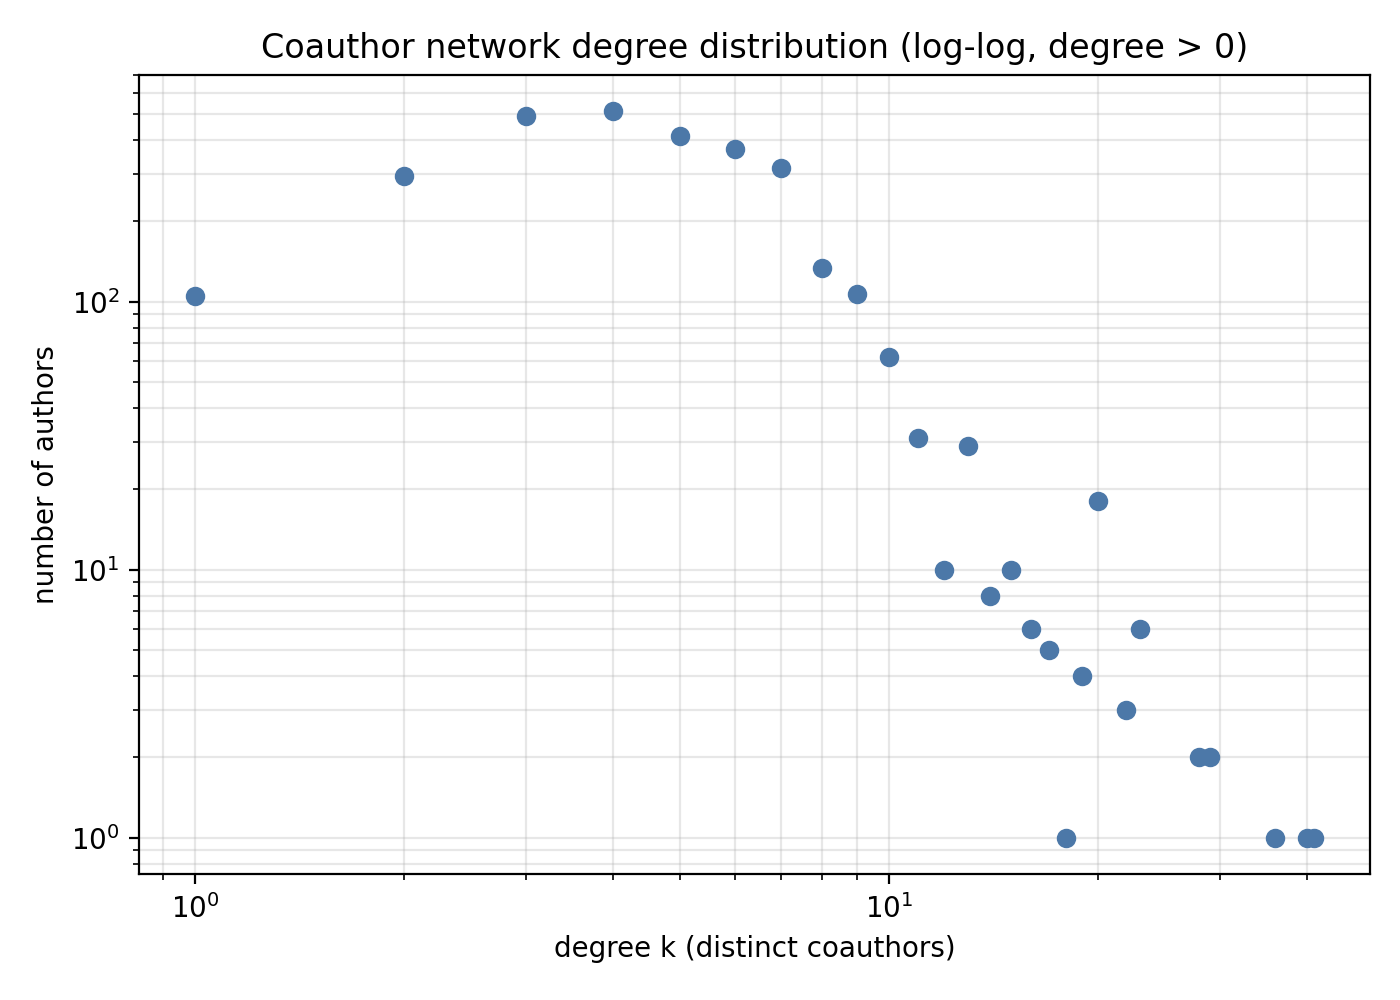
\includegraphics[width=0.92\textwidth]{a_coauthor_degree_loglog.png}
\caption{Phân bố degree của mạng đồng tác giả}
\label{fig:b1}
\end{figure}

Phần lớn tác giả có degree từ 3 đến 7 (nhiều nhất là degree 4, với 514 người); chỉ vài người có degree trên 30. Lý do là mỗi bài tạo ra một nhóm tác giả nối đủ với nhau, nên degree của một người gần bằng tổng số đồng tác giả trên các bài của họ trong mẫu. Hệ số phân cụm cao (0,92) cũng đến từ cấu trúc này.

Mạng rời rạc: thành phần lớn nhất chỉ có 17\% tác giả, còn lại là 411 nhóm nhỏ và 4 người đứng riêng. Đó là hệ quả của cách lấy mẫu (700 bài cố định, không lần theo quan hệ cộng tác), không phản ánh cả cộng đồng Thị giác máy tính. Louvain chia thành phần lớn nhất thành 19 cộng đồng, mỗi cộng đồng 11 đến 41 tác giả. Cộng đồng do thuật toán tìm ra không nhất thiết trùng với một phòng thí nghiệm thật.

\begin{figure}[H]
\centering
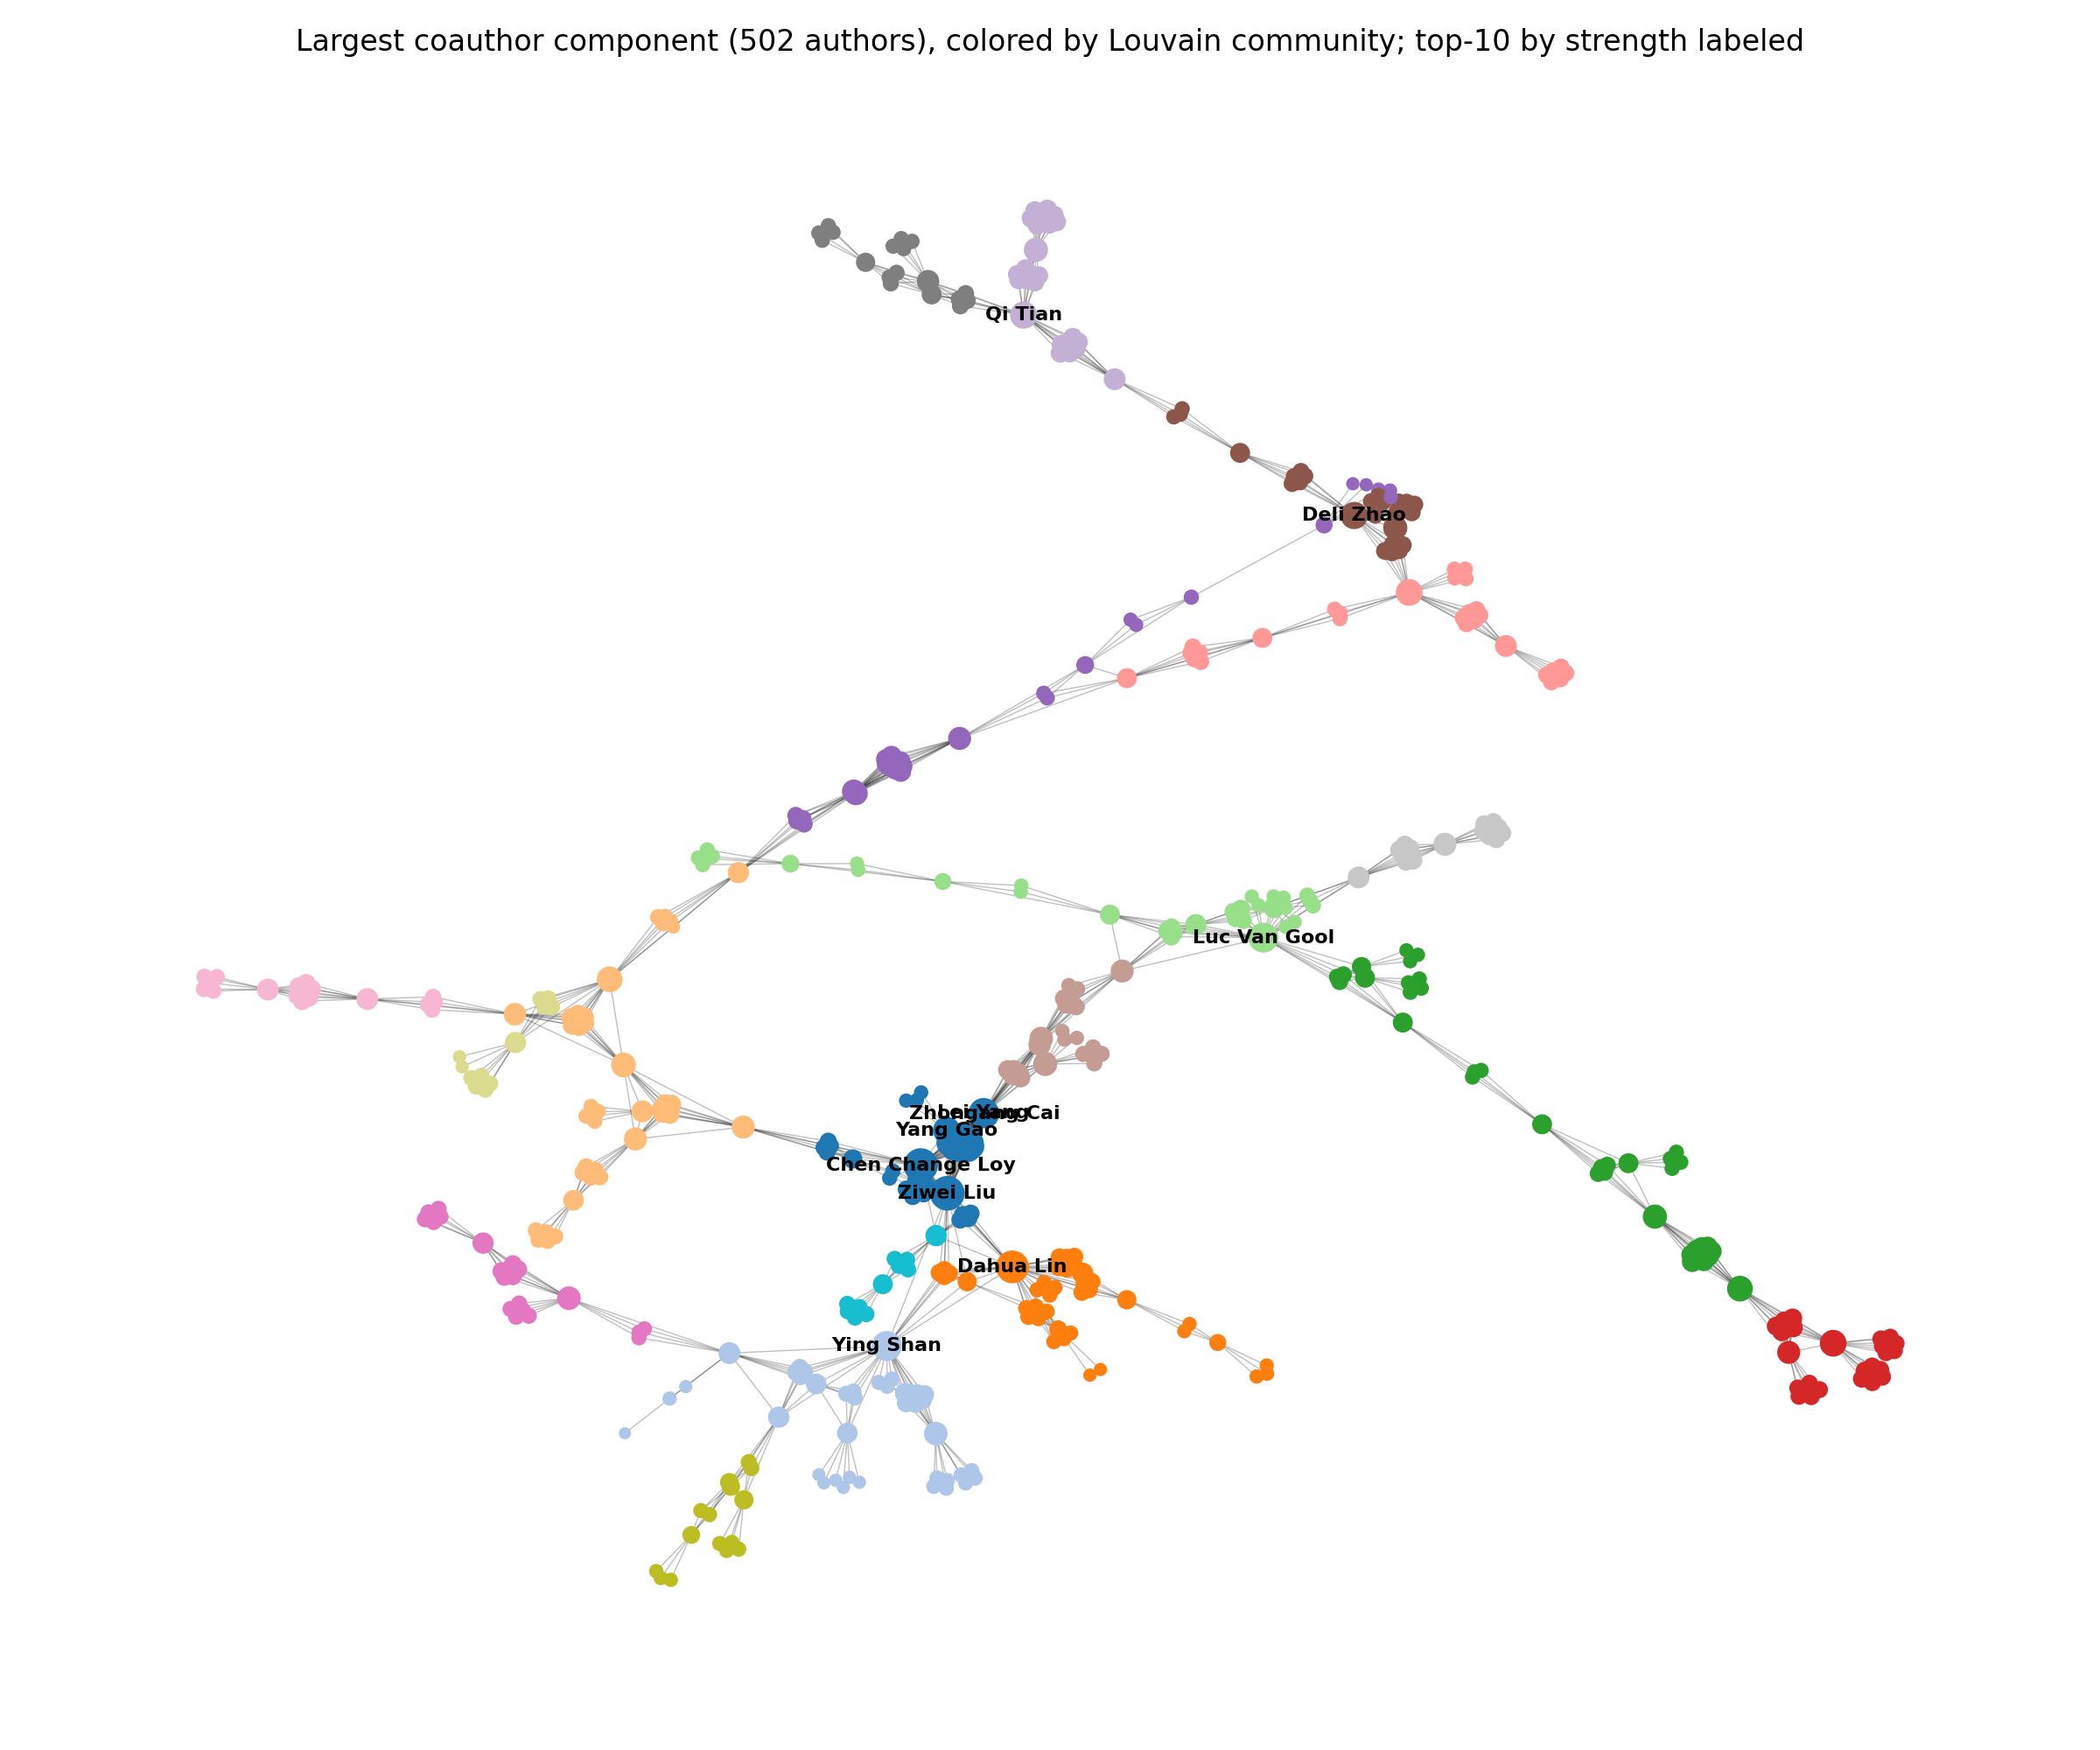
\includegraphics[width=0.92\textwidth]{b_coauthor_lcc_communities.png}
\caption{Thành phần liên thông lớn nhất (502 tác giả), mỗi màu là một cộng đồng Louvain}
\label{fig:b2}
\end{figure}

Năm tác giả có nhiều đồng tác giả nhất là Ziwei Liu (41 người, 5 bài trong mẫu), Chen Change Loy (40 người, 5 bài), Dahua Lin (36 người, 7 bài), Luc Van Gool (29 người, 8 bài) và Ying Shan (29 người, 5 bài). Danh sách này chỉ nói về 700 bài trong mẫu, không phải xếp hạng ảnh hưởng. Một số người có degree cao chỉ vì đứng tên trên bài nhiều tác giả, ví dụ Lei Yang và Zhongang Cai có degree 28 với chỉ 2 bài.

\subsection{Mạng trích dẫn}\label{sec:b5.3}

\begin{table}[H]
\small\centering
\renewcommand{\arraystretch}{1.2}
\caption{Số cạnh trích dẫn theo cặp hội nghị}
\label{tab:b3}
\begin{tabularx}{\textwidth}{@{}>{\raggedright\arraybackslash}X l@{}}
\toprule
\textbf{Bài trích dẫn $\to$ bài được trích dẫn} & \textbf{Số cạnh}\\
\midrule
CVPR 2024 $\to$ ICCV 2023 & 81\\
CVPR 2024 $\to$ CVPR 2024 & 9\\
ICCV 2023 $\to$ ICCV 2023 & 7\\
ICCV 2023 $\to$ CVPR 2024 & 0\\
Tổng & 97\\
\bottomrule
\end{tabularx}
\end{table}

ICCV 2023 diễn ra trước CVPR 2024 nên bài ICCV không thể trích bài CVPR; phần lớn cạnh (81/97) đi theo chiều CVPR sang ICCV. Mạng trích dẫn thưa: 80,3\% bài không trích dẫn và không được trích dẫn bởi bài nào khác trong mẫu. Có 610 thành phần liên thông, chỉ 48 thành phần có từ hai bài trở lên, thành phần lớn nhất gồm 20 bài. Vì vậy mạng này chỉ cho thấy vài cụm nhỏ, chưa đủ để kết luận chung về cách các bài trích dẫn nhau.

\begin{figure}[H]
\centering
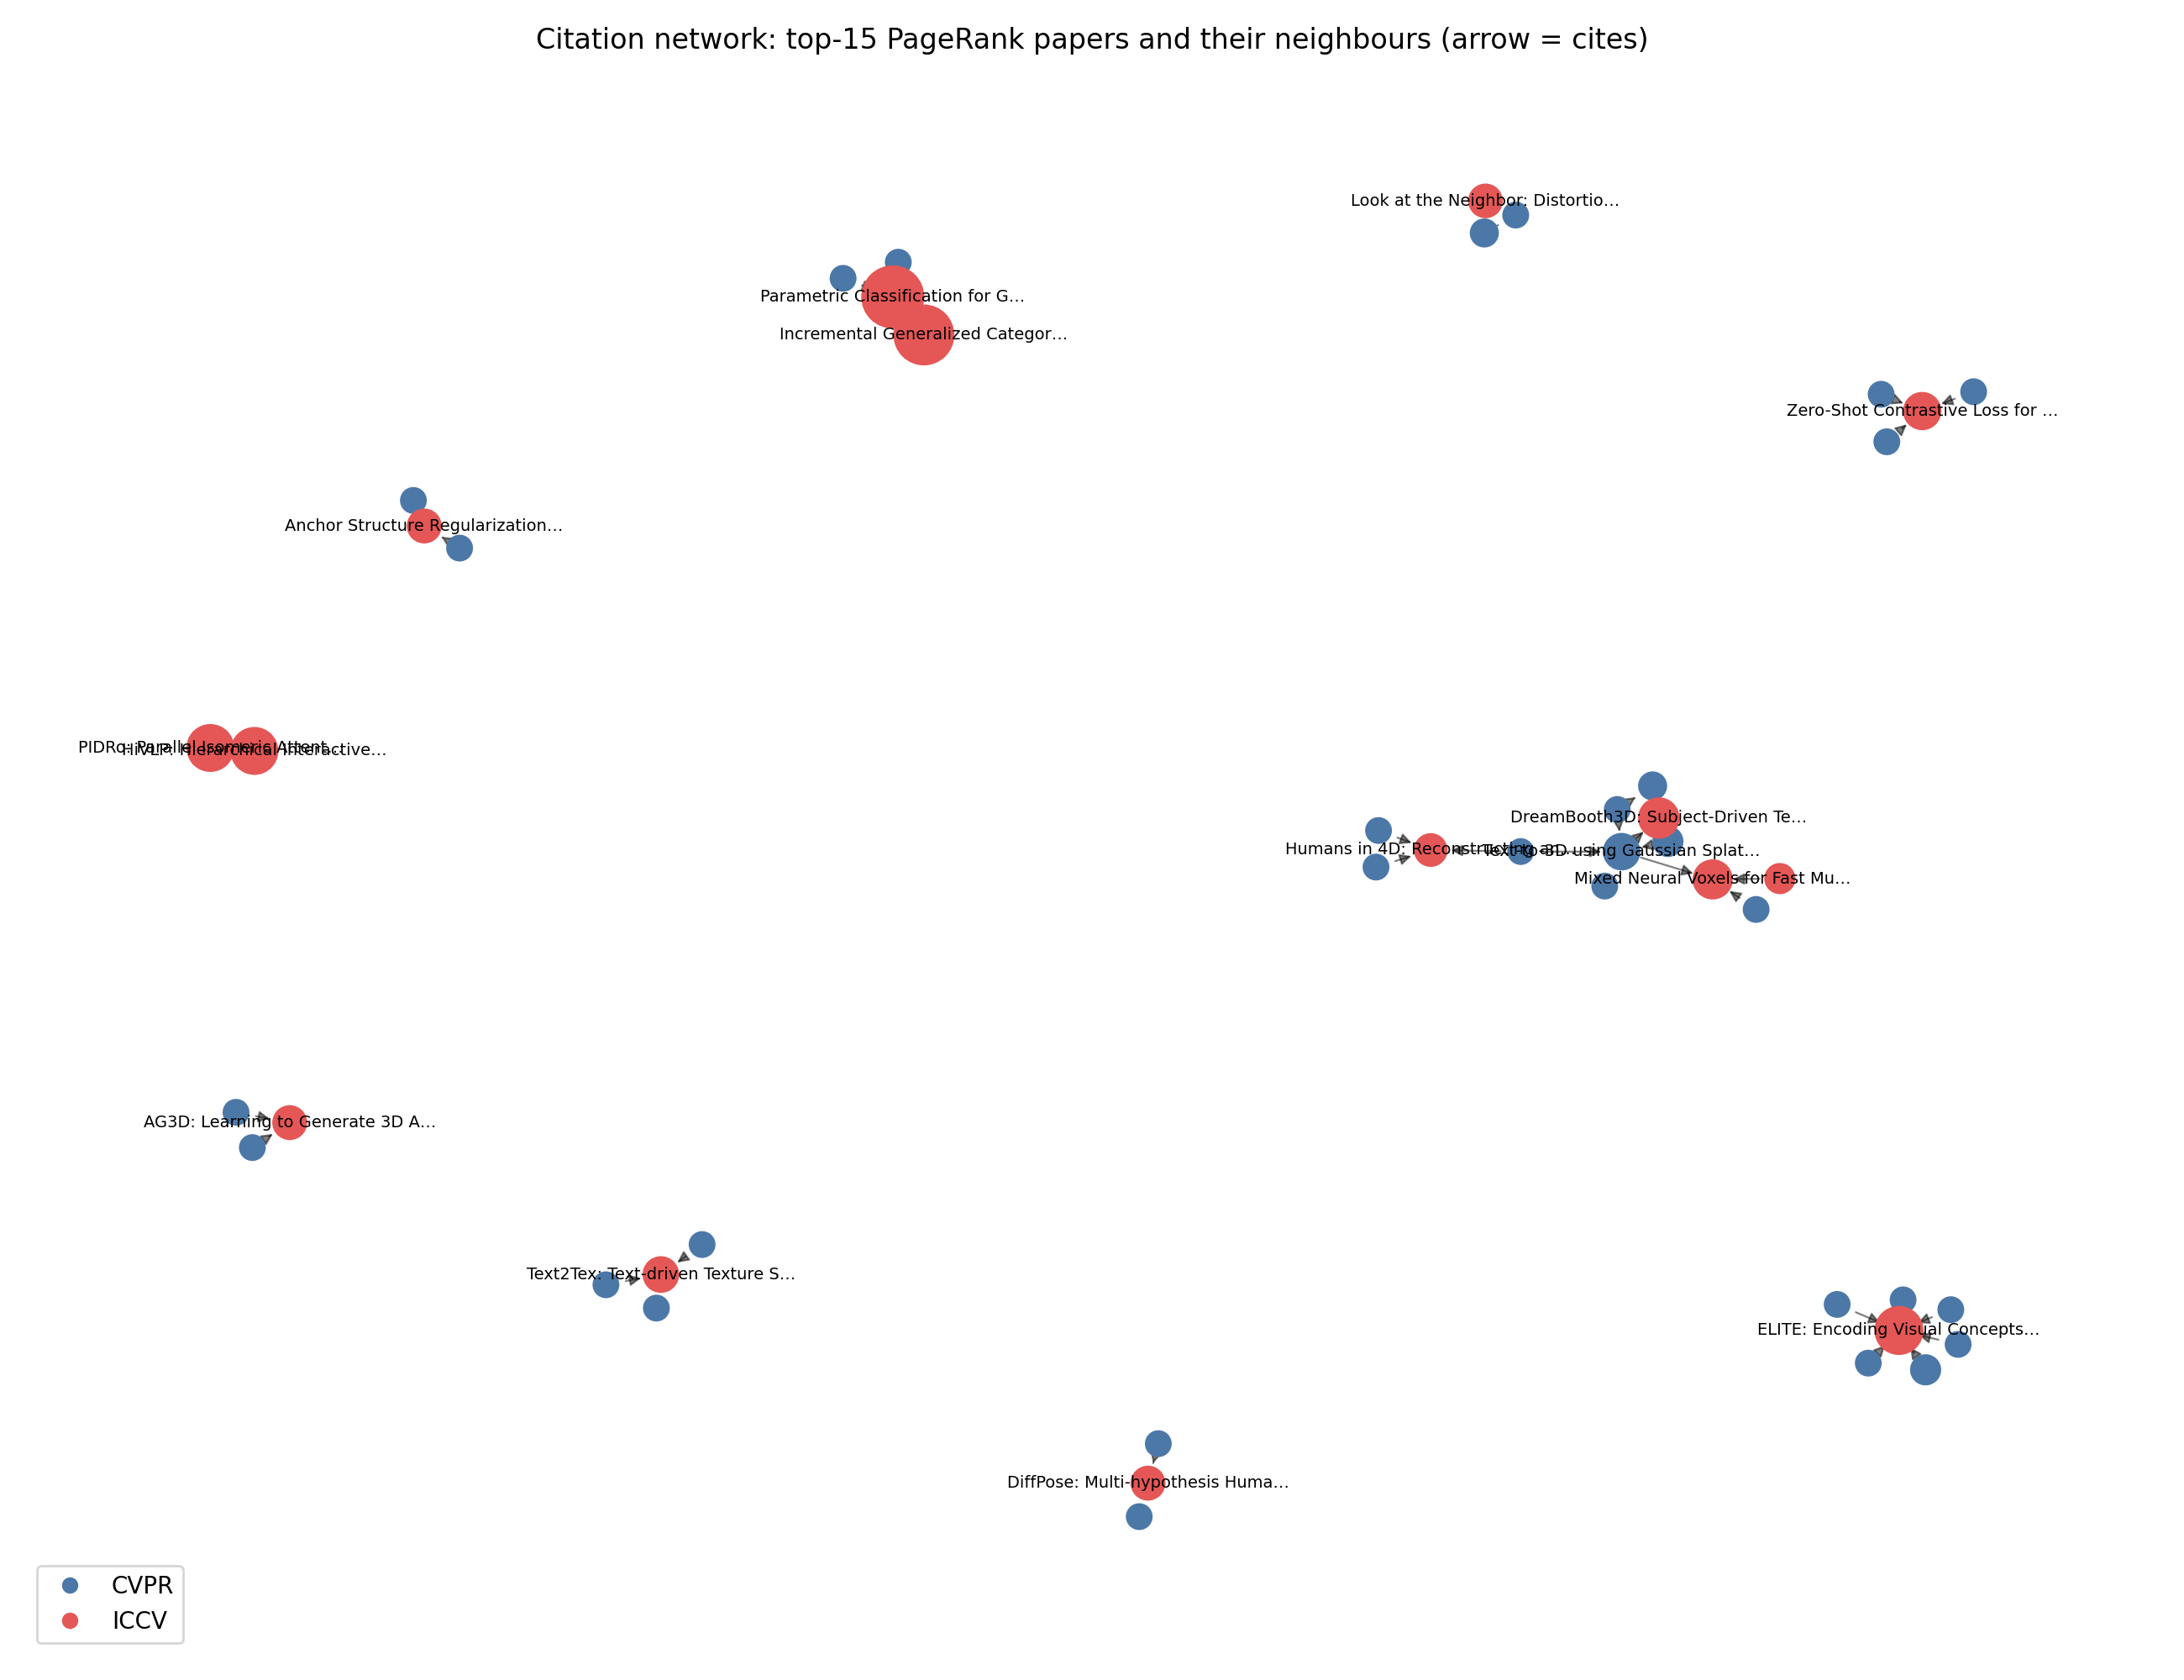
\includegraphics[width=0.92\textwidth]{c_citation_pagerank.png}
\caption{Mạng trích dẫn, kích thước nút theo PageRank}
\label{fig:b3}
\end{figure}

Bài được trích nhiều nhất trong mẫu là ELITE (ICCV 2023, tạo ảnh tùy biến từ văn bản) với 6 lần; tiếp theo là ``Text-to-3D using Gaussian Splatting'' (CVPR 2024) với 4 lần, rồi một số bài ICCV 2023 với 3 lần như Text2Tex, Humans in 4D, DreamBooth3D. Theo PageRank, hai bài đứng đầu là ``Parametric Classification for Generalized Category Discovery'' (0,0154) và ``Incremental Generalized Category Discovery'' (0,0142). Hai bài này không được trích nhiều nhất, chúng có PageRank cao vì nằm trong một cụm nhỏ trích dẫn qua lại. Các con số này chỉ mô tả mẫu, không thay thế được số trích dẫn toàn cầu của bài.

\subsection{Tổ chức và quốc gia}\label{sec:b5.4}

Mạng hợp tác tổ chức có 432 tổ chức và 1140 cạnh, trong đó 26 tổ chức không hợp tác với ai trong mẫu. Quốc gia của một bài là tập quốc gia của các tổ chức mà tác giả ghi trên bài đó. 666/700 bài xác định được ít nhất một quốc gia; 34 bài còn lại không được tính trong các thống kê theo quốc gia.

\begin{table}[H]
\footnotesize\centering
\renewcommand{\arraystretch}{1.2}
\caption{Tổ chức hợp tác nhiều nhất (trái) và quốc gia có nhiều bài nhất (phải)}
\label{tab:b4}
\begin{tabularx}{\textwidth}{@{}>{\raggedright\arraybackslash}X l l @{\hspace{1.2cm}} l l l@{}}
\toprule
\textbf{Tổ chức (nước)} & \textbf{Degree} & \textbf{Strength} & \textbf{Quốc gia} & \textbf{Số tổ chức} & \textbf{Số bài}\\
\midrule
Tsinghua University (CN) & 48 & 69 & CN & 111 & 342\\
Zhejiang University (CN) & 38 & 54 & US & 98 & 206\\
Peking University (CN) & 32 & 52 & HK & 7 & 60\\
Alibaba Group (CN) & 29 & 47 & KR & 24 & 53\\
Shanghai AI Laboratory (CN) & 30 & 46 & SG & 8 & 49\\
Chinese Academy of Sciences (CN) & 24 & 44 & GB & 19 & 47\\
\bottomrule
\end{tabularx}
\end{table}

{\footnotesize Degree: số tổ chức khác đã viết chung. Strength: tổng số bài chung với các tổ chức đó. Số bài của quốc gia: số bài có ít nhất một tổ chức ở nước đó.\par}

\begin{figure}[H]
\centering
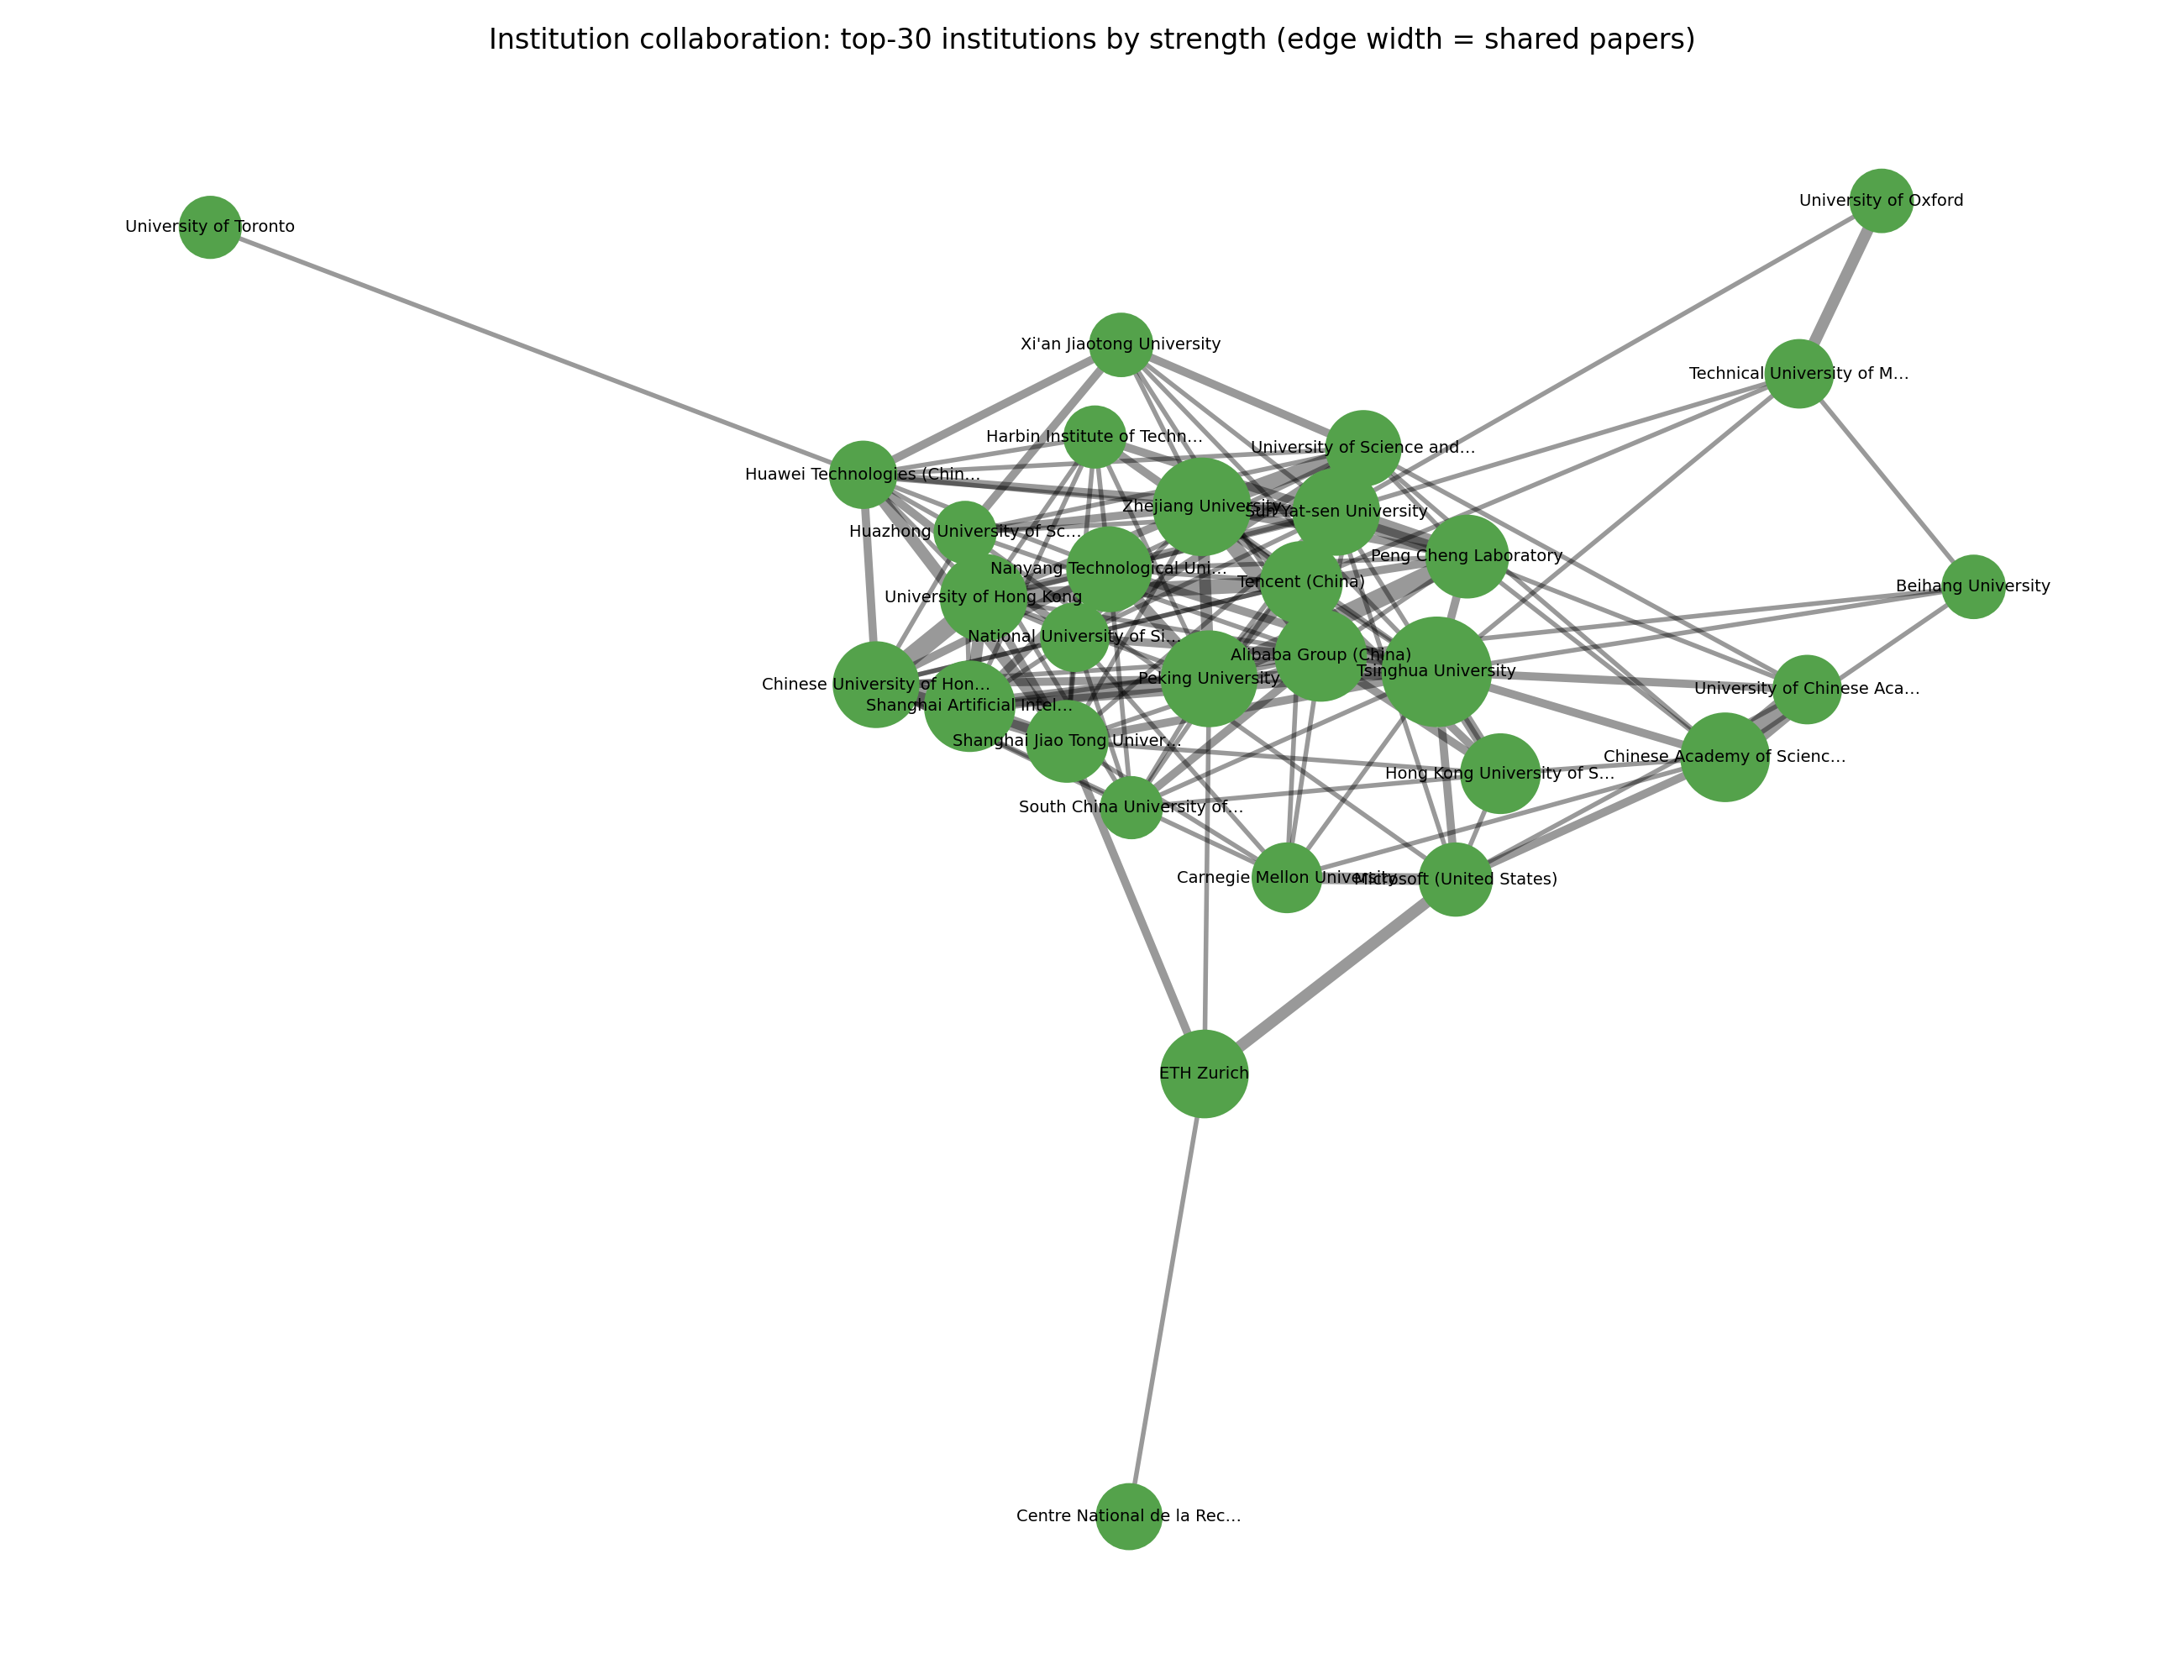
\includegraphics[width=0.92\textwidth]{d_institution_collaboration_top30.png}
\caption{Mạng hợp tác của 30 tổ chức có strength cao nhất; cạnh càng dày, càng nhiều bài chung}
\label{fig:b4}
\end{figure}

Một số cặp hợp tác mạnh nhất thực ra là các đơn vị cùng một hệ thống, ví dụ Chinese Academy of Sciences với Institute of Automation (8 bài) hay với University of Chinese Academy of Sciences (7 bài).

Quy về cấp quốc gia, tổng trọng số hợp tác trong cùng một nước là 686 và giữa hai nước khác nhau là 664, trải trên 111 cặp quốc gia. Các cặp quốc tế mạnh nhất là \textbf{CN--US (99), CN--HK (83), CN--SG (46)}, sau đó CN--AU (30), HK--US (24), CN--GB (19). Nói cách khác, hợp tác quốc tế trong mẫu chủ yếu là giữa Trung Quốc đại lục với Mỹ, Hồng Kông và Singapore.

\subsection{Trích dẫn giữa các quốc gia}\label{sec:b5.5}

Trong 97 cạnh trích dẫn, 95 cạnh xác định được quốc gia ở cả hai đầu. Mỗi cạnh có tổng trọng số 1, chia đều cho mọi cặp (nước của bài trích dẫn, nước của bài được trích dẫn). Như vậy một bài nhiều nước không làm số trích dẫn tăng lên. Đây là phép tổng hợp trên các cạnh có sẵn, không thêm quan hệ mới vào graph.

\begin{table}[H]
\small\centering
\renewcommand{\arraystretch}{1.2}
\caption{Trích dẫn giữa các quốc gia (6 cặp lớn nhất, tổng trọng số 95)}
\label{tab:b5}
\begin{tabularx}{\textwidth}{@{}l l >{\raggedright\arraybackslash}X@{}}
\toprule
\textbf{Nước bài trích dẫn} & \textbf{Nước bài được trích} & \textbf{Trọng số}\\
\midrule
CN & CN & 19,28\\
US & US & 7,17\\
CN & HK & 5,36\\
CN & US & 5,36\\
DE & CN & 4,33\\
US & CN & 3,42\\
\bottomrule
\end{tabularx}
\end{table}

Trích dẫn trong cùng một nước chiếm 30,78 (32,4\%), giữa hai nước khác nhau chiếm 64,22 (67,6\%). Tỷ lệ giữa hai nước bị đẩy lên phần nào do cách chia đều khi bài có nhiều nước. Trung Quốc tự trích dẫn nhiều nhất (19,28), sau đó là Mỹ (7,17). Với chỉ 95 cạnh, bảng này cho thấy xu hướng chứ chưa đủ để so sánh giữa các nước nhỏ.

\subsection{Task và Method phổ biến}\label{sec:b5.6}

\begin{figure}[H]
\centering
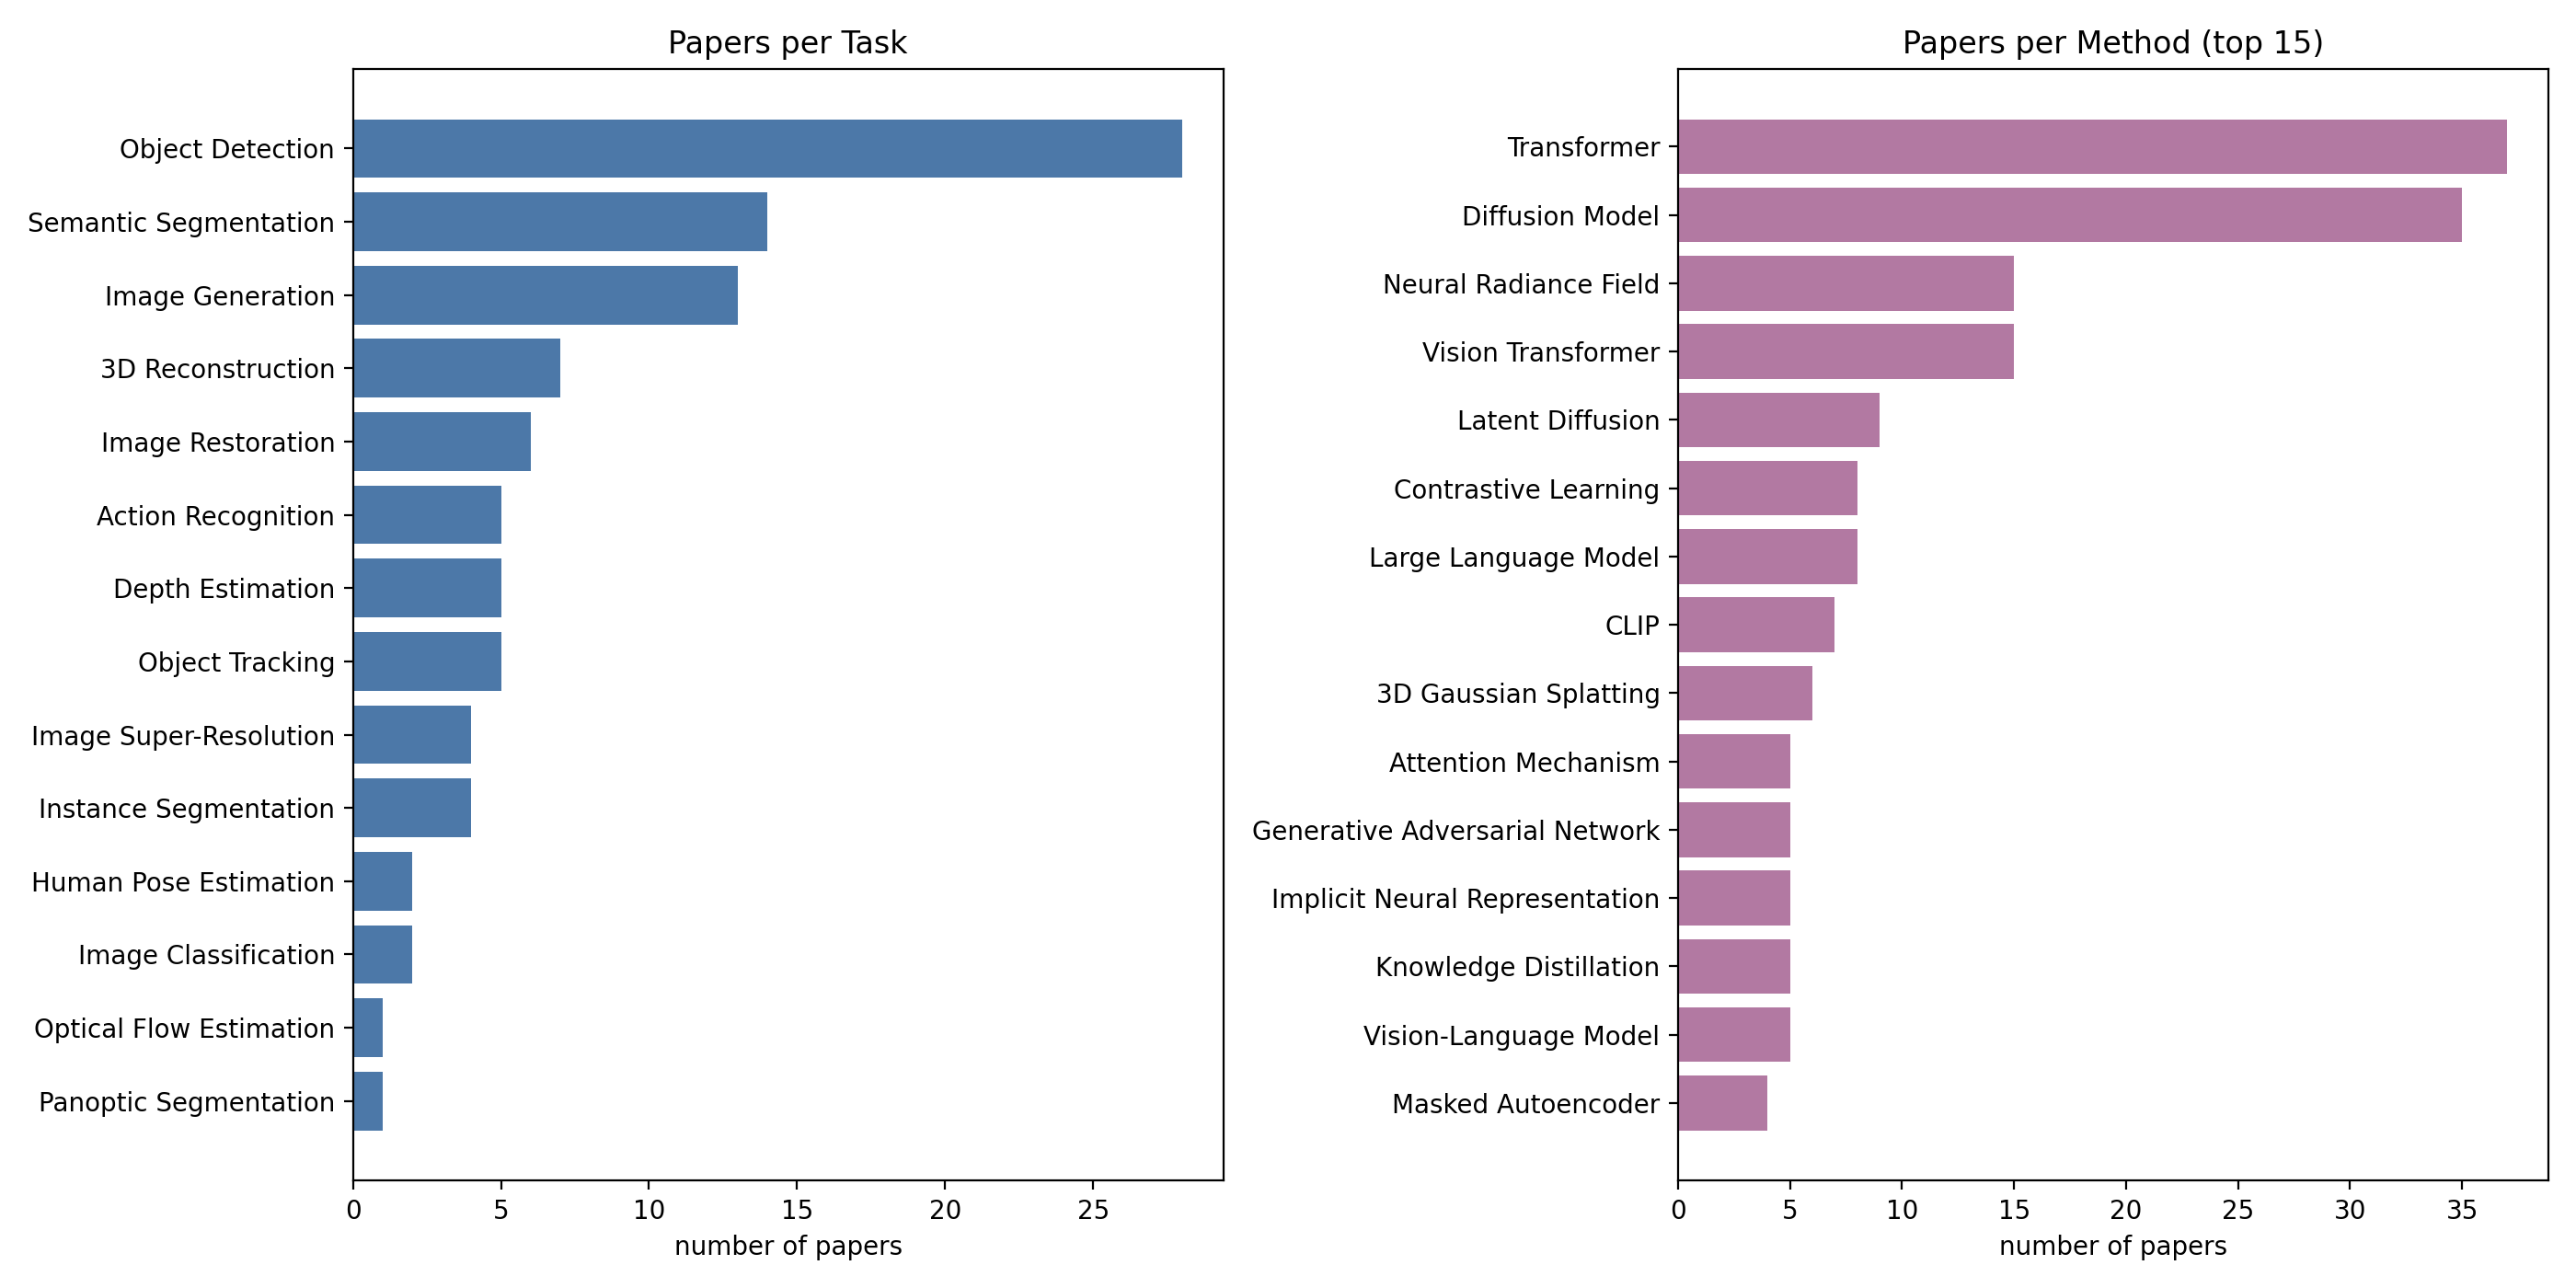
\includegraphics[width=0.92\textwidth]{f_task_method_counts.png}
\caption{Số bài theo Task và theo Method}
\label{fig:b5}
\end{figure}

Về Task, Object Detection nhiều nhất với 28 bài, sau đó là Semantic Segmentation (14), Image Generation (13), 3D Reconstruction (7) và Image Restoration (6). Về Method, Transformer (37 bài) và Diffusion Model (35) dẫn đầu, tiếp theo là Neural Radiance Field và Vision Transformer (15 bài mỗi loại), Latent Diffusion (9), Contrastive Learning và Large Language Model (8 mỗi loại). Dataset được nhận nhiều nhất là nuScenes (6 bài), COCO và KITTI (3 bài mỗi loại).

Chỉ 95 bài có Task, 178 bài có Method và 21 bài có Dataset; tổng cộng 267 bài có ít nhất một cạnh NLP. 433 bài còn lại không phải là không thuộc Task nào, mà luật chưa nhận ra (Mục~\ref{sec:nlp}). Thứ hạng ở đây vì vậy chỉ là gần đúng.

\subsection{Case study: Object Detection}\label{sec:b5.7}

Nhóm chọn Object Detection vì đây là Task có nhiều bài nhất (28 bài: 20 ICCV, 8 CVPR). Mạng con gồm nút Task, cả 28 bài, các Method và Dataset của các bài đó, rồi thêm tác giả (ưu tiên người có nhiều bài hơn) và tổ chức liên quan cho tới khi đủ 80 nút. Kết quả là \textbf{80 nút} (28 Paper, 25 Author, 20 Institution, 4 Method, 2 Dataset, 1 Task) và \textbf{98 cạnh}.

\begin{figure}[H]
\centering
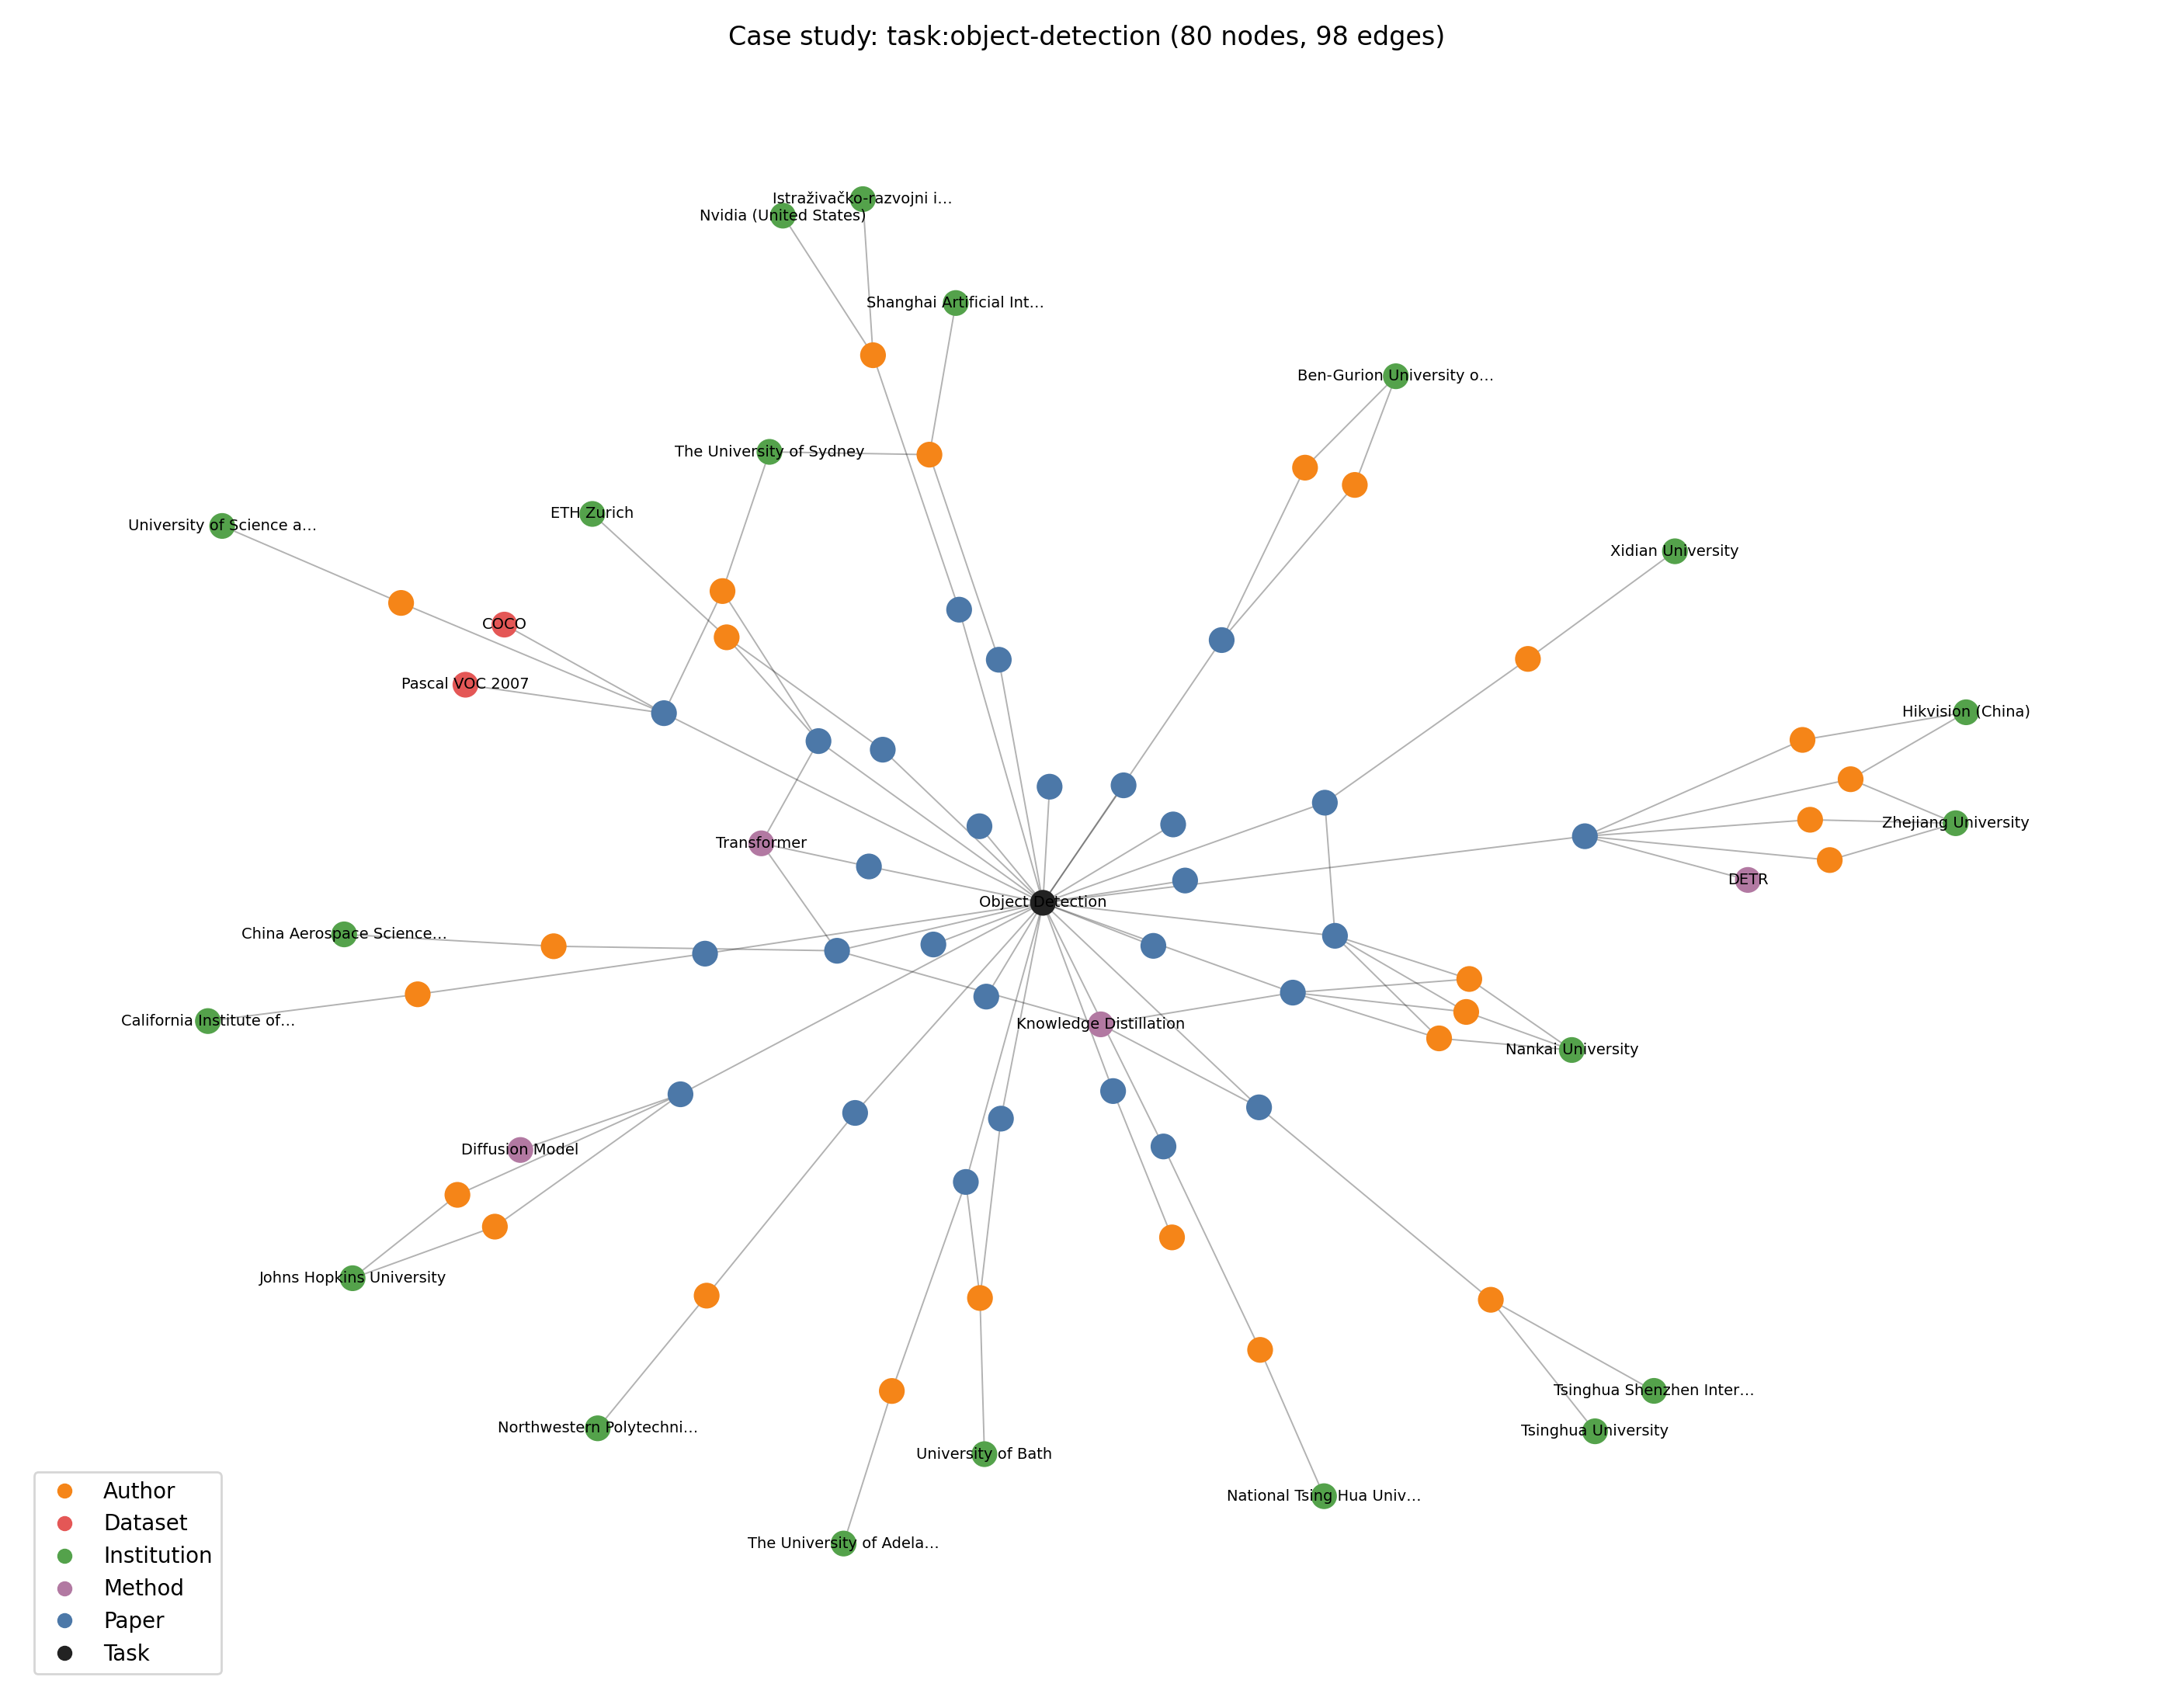
\includegraphics[width=0.92\textwidth]{e_case_study.png}
\caption{Mạng con quanh Task Object Detection}
\label{fig:b6}
\end{figure}

Các Method xuất hiện là DETR, Diffusion Model, Knowledge Distillation và Transformer; Dataset là COCO và Pascal VOC 2007. Tổ chức gồm Tsinghua University, Zhejiang University, ETH Zurich, Nvidia, Shanghai AI Laboratory, Hikvision và một số nơi khác (20 tổ chức). Không ai trong 25 tác giả có quá 2 bài, nên quanh Task này không có nhóm tác giả hợp tác dày.

Mạng con chỉ có \textbf{một cạnh trích dẫn} (một bài CVPR 2024 về phát hiện đối tượng trên ảnh SAR trích một bài ICCV 2023 về ảnh viễn thám). Các bài còn lại nối riêng lẻ vào nút Task, tạo hình ngôi sao. Mạng con cho biết ai làm Object Detection và dùng gì, nhưng không cho thấy các nhóm này hợp tác hay trích dẫn nhau. Điều này khớp với việc mạng trích dẫn chung rất thưa.

\subsection{Truy vấn Cypher minh họa}\label{sec:b5.8}

Đếm trích dẫn theo cặp hội nghị:
{\small
\begin{verbatim}
MATCH (a:Paper {project_id: 'mxh_cv_700'})-[:CITES]->(b:Paper)
RETURN a.conference AS citing_conference, b.conference AS cited_conference, count(*) AS citations
ORDER BY citing_conference, cited_conference;
\end{verbatim}}
Kết quả gồm 3 dòng (CVPR$\to$CVPR 9, CVPR$\to$ICCV 81, ICCV$\to$ICCV 7), khớp Bảng~\ref{tab:b3}.

Các bài được trích nhiều nhất trong mẫu:
{\small
\begin{verbatim}
MATCH (:Paper {project_id: 'mxh_cv_700'})-[c:CITES]->(p:Paper)
RETURN p.name AS title, p.conference AS conference, count(c) AS cited_by_core
ORDER BY cited_by_core DESC, title
LIMIT 15;
\end{verbatim}}
Kết quả gồm 15 dòng, đứng đầu là ELITE với 6 lần.



\section{Kết luận}

\subsection{Kết quả đạt được}
\begin{itemize}[leftmargin=1.4em]
  \item Graph có 4182 nút và 16979 cạnh với 8 loại nút và 10 loại quan hệ, vượt yêu cầu 2000 nút, 5000 cạnh. Nhóm không thêm bài ngoài mẫu để tăng số lượng.
  \item Cạnh nào cũng có nguồn gốc kiểm tra được; cạnh NLP có câu gốc và luật đã dùng.
  \item Chấm mẫu cho 99/100 cạnh đúng, ước lượng có trọng số 98,1\%.
  \item Graph lưu trong Neo4j, nạp lại không sinh trùng; toàn bộ quy trình chạy lại được offline.
  \item Đã phân tích mạng đồng tác giả, trích dẫn, hợp tác tổ chức và quốc gia, trích dẫn giữa các nước, Task/Method phổ biến và một case study 80 nút.
\end{itemize}

\subsection{Hạn chế}
\begin{table}[H]
\small\centering
\renewcommand{\arraystretch}{1.25}
\caption{Các hạn chế chính}
\label{tab:hanche}
\begin{tabularx}{\textwidth}{@{}>{\raggedright\arraybackslash}p{3.2cm} >{\raggedright\arraybackslash}X@{}}
\toprule
\textbf{Vấn đề} & \textbf{Chi tiết}\\
\midrule
Thiếu tác giả & 539/4384 dòng dữ liệu tác giả (12,3\%) không vào graph do chưa xác định được danh tính; 24 bài (23 bài CVPR) không có tác giả nào vì không tìm thấy trên OpenAlex. Mạng đồng tác giả vì thế thiếu cạnh.\\
Gán nhầm tổ chức & OpenAlex ghép nhầm một số tổ chức trùng tên ở nước khác, ví dụ Korea University (Hàn Quốc) với một trường cùng tên ở Nhật, Southeast University (Trung Quốc) với trường cùng tên ở Bangladesh. Lỗi này kéo theo cạnh hợp tác và thống kê quốc gia sai.\\
Tổ chức mẹ/con tách riêng & Ví dụ Chinese Academy of Sciences và Institute of Automation là hai nút, nên cạnh hợp tác mạnh nhất (8 bài) thực chất là nội bộ một hệ thống.\\
Một người hai ID & 38 cặp tác giả cùng tên và cùng tổ chức hoặc cùng đồng tác giả, nhiều khả năng là một người (ví dụ Michael J. Black, Liang Lin, Bo Dai); 3 ORCID xuất hiện trên hai nút.\\
Trích dẫn thưa & Chỉ 97 cạnh vì mỗi hội nghị lấy 350 bài và không thêm bài ngoài mẫu. 80,3\% bài không có cạnh trích dẫn nào.\\
NLP bỏ sót & Chỉ 267/700 bài có cạnh NLP. ImageNet được nhắc trong 42 bài nhưng chỉ 6 bài có cạnh EVALUATED\_ON. Có vài lỗi nghĩa, ví dụ SAM (Sharpness-Aware Minimization) bị nhận thành Segment Anything Model; và vài Dataset trùng nghĩa (COCO và COCO 2017).\\
Mẫu và thuật toán & 700 bài cố định không đại diện cho cả ngành. Kết quả Louvain có thể đổi khi đổi phiên bản thư viện hoặc seed. Mẫu chấm 100 cạnh đủ để phát hiện loại lỗi chính, chưa đủ để ước lượng chặt từng loại quan hệ.\\
\bottomrule
\end{tabularx}
\end{table}

\subsection{Hướng khắc phục}
Theo thứ tự ưu tiên:
\begin{enumerate}[leftmargin=1.6em]
  \item So tổ chức trên OpenAlex với tên tổ chức và quốc gia ghi trên bài để loại các ghép nhầm trùng tên.
  \item Gộp tổ chức con về tổ chức mẹ (dùng quan hệ mẹ/con của ROR) trước khi tạo cạnh hợp tác.
  \item Gộp các tác giả trùng ORCID, hoặc trùng tên cùng tổ chức và cùng đồng tác giả.
  \item Bổ sung ID cho tác giả còn thiếu bằng danh sách tác giả trên CVF kết hợp ORCID.
  \item Mở rộng mẫu hoặc thêm có kiểm soát các bài tham khảo được trích nhiều để mạng trích dẫn dày hơn.
  \item Mở rộng từ điển và nới luật NLP, kiểm chứng lại bằng mẫu chấm.
\end{enumerate}
\newpage

\section*{Tài liệu tham khảo}
\addcontentsline{toc}{section}{Tài liệu tham khảo}
\begin{enumerate}[leftmargin=2em, label={[\arabic*]}]
  \item CVF Open Access. \url{https://openaccess.thecvf.com/}
  \item OpenAlex, Works và Authorships. \url{https://help.openalex.org/data/works/}, \url{https://help.openalex.org/data/authorships/}
  \item arXiv, Version control. \url{https://info.arxiv.org/help/versions.html}
  \item Crossref REST API. \url{https://www.crossref.org/documentation/retrieve-metadata/rest-api/}
  \item spaCy, Rule-based matching. \url{https://spacy.io/usage/rule-based-matching}
  \item Neo4j Documentation. \url{https://neo4j.com/docs/}
  \item NetworkX Documentation. \url{https://networkx.org/documentation/stable/}
\end{enumerate}

\end{document}
